\documentclass[12pt,letterpaper]{report}
\usepackage[margin=1in,includeheadfoot]{geometry}
\usepackage[hidelinks,bookmarksnumbered]{hyperref}
\usepackage[figure,table]{hypcap}
\usepackage[nottoc]{tocbibind}
\usepackage[titletoc]{appendix}
\usepackage[utf8]{inputenc}
\usepackage[T1]{fontenc}
\usepackage{todonotes}
\usepackage{algorithm}
\usepackage{algpseudocode}
\usepackage{subfig}

\usepackage{fancyhdr}
\pagestyle{fancy}
\fancyhf{}
\rhead{\textit{\leftmark}}
\cfoot{\thepage}
\renewcommand{\headrulewidth}{0pt}

\usepackage[backend=biber,sorting=none]{biblatex}
\addbibresource{references.bib}

\usepackage{graphicx}
\graphicspath{ {images/} }

\usepackage{setspace}
\doublespacing

\usepackage{datetime}
\newdateformat{monthyeardate}{\monthname[\THEMONTH] \THEYEAR}
\newdateformat{yeardate}{\THEYEAR}

\usepackage{sectsty}
\chapterfont{\vspace*{-17.5mm}\large\sc\centering}
\chaptertitlefont{\centering}
\subsubsectionfont{\centering}

\newcommand*{\cls}{\fontfamily{cmss}\selectfont}

\newcommand{\jkReplace}[2]{\textcolor{red}{JK replaced: }\textcolor{blue}{#1}{\textcolor{red}{\ by }\textcolor{green}{#2}}}

%----------------
% Title Page
%----------------
\begin{document}

\begin{titlepage}
	\begin{center}
		\vspace*{1in}
		
		\Huge
		Concern-Oriented Use Case Maps
		
		\vfill
		
		\large
		Cheuk Chuen Siow\\
		School of Computer Science\\
		McGill University, Montréal
		
		\vfill
		
		\monthyeardate\today
		
		\vfill
		
		A thesis submitted to McGill University in partial fulfillment of the requirements for the degree of Master of Science in Computer Science
		
		\vfill
		
		\textcopyright{} Cheuk Chuen Siow \yeardate\today
		
		\vspace*{1in}
	\end{center}
\end{titlepage}

%----------------
% Front Matter
%----------------
\clearpage
\pagenumbering{roman}
\setcounter{page}{2}

\chapter*{Abstract}
\addcontentsline{toc}{chapter}{Abstract}

Concern-Oriented Reuse (CORE) is a reuse paradigm that extends model-driven engineering with advanced modularization, goal modeling, and software product lines. Previous work enables modeling with CORE at the design level using Reusable Aspect Models (RAM). Requirements elicitation is also a crucial aspect of software development process, and one of the visual notation that expresses use cases as graphical workflows is Use Case Maps (UCM). UCM bridges the gap between requirements and design, and is part of the User Requirements Notation (URN) for scenario modeling. This thesis addresses the need for enabling scenario modeling in CORE. Based on Aspect-Oriented Use Case Maps (AoUCM), we introduce a novel technique that applies advanced separation of concerns for model-driven requirements elicitation with use cases---Concern-Oriented Use Case Maps (CoUCM). We define a metamodel for CoUCM that derives from the CORE metamodel, and formulate the weaving algorithm for CoUCM model composition. We then implement CoUCM in the TouchCORE tool as proof of concept. We present a working application of scenario modeling with TouchCORE, in which we further validate our implementation through case studies and workflow patterns. Validation shows that CoUCM is able to model requirements concerns that are reusable and scalable, and that further work is required to provide a more comprehensive implementation of CoUCM.

\clearpage

\chapter*{Abrégé}
\addcontentsline{toc}{chapter}{Abrégé}



\clearpage

\chapter*{Acknowledgements}
\addcontentsline{toc}{chapter}{Acknowledgements}



\clearpage

\chapter*{Preface}
\addcontentsline{toc}{chapter}{Preface}



% Content
\renewcommand{\contentsname}{Table of Contents}
\tableofcontents
\listoffigures
%\listoftables
\listofalgorithms

\clearpage
\pagenumbering{arabic}

%----------------
% Main Body
%----------------
\chapter{Introduction}
% !TEX root = ../thesis.tex

Since 1960s, software development has been evolving rapidly to address the increasing demands of complex software. The complexity of modern software brings about difficulties in developing and maintaining quality software. Software engineering as a discipline ensures that developers follow a systematic production of software, by applying best practices to maximize quality of deliverables and minimize time-to-market. Various methodologies exist through the efforts of active research by theorists and practitioners, but the core of software development process typically consists of the following six phases---requirements gathering, design, implementation, testing, deployment, and maintenance.

Conceptual models help illustrates complex systems with a simple framework by creating abstractions to alleviate the amount of complexity. Hence, the use of models is progressively recommended in representing a software system. This simplifies the process of design, maximizes compatibility between different platforms, and promotes communication among stakeholders. Model-Driven Engineering (MDE) technologies offer the means to represent domain-specific knowledge within models, allowing modelers to express domain concepts effectively~\cite{schmidt2006model}. MDE advocates using the best modeling formalism that expresses relevant design intent declaratively at each level of abstraction. During development, we can use models to describe different aspects of the system vertically, in which the models are refined from higher to lower levels of abstraction through model transformation. At the lowest level, models use implementation technology concepts, and appropriate tools can be used to generate code from these platform-specific models~\cite{sendall2003model}.

Modularity is key in designing computer programs that are extensible and easily maintainable, but concerns that are crosscutting and more scattered in the implementation are more likely to cause defects~\cite{eaddy2008crosscutting}. This poses obstacles for MDE because modeling such crosscutting concerns in a modular way is difficult from an object-oriented standpoint. Furthermore, reusability is also a main factor in allowing developers to leverage reusable solutions such as libraries and frameworks provided for a given programming language, thereby improving the development speed without having to implement existing software components from first principles. Model reuse is still in its early stage, but modeling libraries are emerging as well~\cite{france2012repository}.

Concern-Oriented Reuse (CORE) is a new software development paradigm or approach that puts reuse at the forefront of software development~\cite{alam2013concern}. In CORE, software development is structured around modules called \emph{concerns} that provide a variety of reusable solutions for recurring software development issues. Techniques from MDE, Software Product Lines (SPL) engineering, and software composition (in particular feature-orientation and aspect-orientation) allow concerns to form modular units of reuse that encapsulate a set of software development artifacts, i.e., models and code, during software development in a versatile, generic way.

The main premise of CORE is that recurring development concerns are made available in a concern library, which eventually should cover most recurring software development needs. Similar to class libraries in modern programming languages, this library should grow as new development concerns emerge, and existing concerns should continuously evolve as alternative architectural, algorithmic, and technological solutions become available. Applications are built by reusing existing concerns from the library whenever possible, following a well-defined reuse process supported by clear interfaces. To generate an executable in which concerns exhibit intricate crosscutting structure and behavior, CORE relies on additive software composition techniques, feature-oriented technology, and aspect-oriented technology.

Currently, CORE only supports modelling notations that are used at the design phase~\cite{kienzle2010aspect}. In order to fully integrate CORE with MDE, other development phases should also be supported. We are interested in adding support for requirements modeling languages to CORE, so that requirements modellers too can benefit from advanced modularization and reuse support. We chose to concentrate on the User Requirements Notation (URN), which sets the standard as a visual notation for modeling and analyzing requirements~\cite{amyot2002urn}. URN formalizes and integrates two complementary languages: (i) Goal-oriented Requirements Language (GRL) to describe non-functional requirements as intentional elements, and (ii) Use Case Map (UCM) to describe functional requirements as causal scenarios. GRL and UCM are used to capture goal and scenario models, respectively. Since CORE already supports the use of goal models to analyze the impact of choosing features~\cite{alam2013concern}, this thesis focuses on integrating scenario models with the concepts of CORE.

\section{Contributions}

This thesis advances the state-of-the-art in modeling by proposing a complete solution for augmenting the UCM modeling notation with CORE capabilities, resulting in a variant of UCM---Concern-Oriented Use Case Maps (CoUCM). Specifically, the thesis makes the following contributions:

\begin{itemize}

\item A metamodel for CoUCM that extends the CORE metamodel, thus formalizing the integration of the CORE concepts into the UCM language.

\item A CORE-compatible weaving algorithm for CoUCMs that takes as an input two CoUCM models and produces a composed CoUCM model. This makes it possible for requirements engineers to modularize scenarios according to concern features (i.e., a weaving algorithm compatible with CORE extension) as well as to reuse existing scenarios when creating new ones (i.e., compatible with the CORE reuse mechanism).

\item An implementation of the proposed CoUCM metamodel and weaving algorithm in TouchCORE, serving as a proof of concept validation.

\item A demonstration of the expressiveness and reuse potential of CoUCMs by means of an \emph{Authentication} concern and an \emph{Online Payment} concern, and two \emph{Workflow Patterns} case studies.

\end{itemize}

\section{Thesis Outline}

The remainder of this thesis is structured as follows. Chapter~\ref{ch:2} offers background information on CORE and UCM, as well as presents existing modeling techniques closely related to our work. Chapter~\ref{ch:3} details the integration of CORE with UCM, namely the CoUCM meta model and the different CoUCM weaving algorithms. Chapter~\ref{ch:4} validates the proposed meta model
and weaving algorithms by presenting some details of the TouchCORE implementation. Finally, Chapter~\ref{ch:5} concludes the thesis and discusses possible future work.


\chapter{Background} \label{ch:2}
First paragraph opens with URN and its components.

\section{Use Case Map (UCM)}

This section describes UCM in detail.

\section{Concern-oriented Reuse (CORE)}

This section describes CORE in detail.

\subsection{Reusable Aspect Models (RAM)}

\section{Overview of Relevant Modeling Tools}

Literature review.

\section{Motivation}

Build on the motivation of having UCM as an additional model for TouchCORE.

\subsection{UCM in the Context of CORE}

Weaving, extending, and reusing UCM concern models.

Last paragraph leads to implementation chapter.


\chapter{Adding Support for UCM to CORE} \label{ch:3}
% !TEX root = ../thesis.tex

Although hypothetically CORE offers a base that supports multiple modeling languages, only one notation has been integrated with CORE thus far---the RAM modeling notation that is used for design modeling with class, sequence, and state diagrams~\cite{kienzle2010aspect, klein2007reusable}. The goal of the thesis is to investigate whether CORE can also support an additional modeling language---the requirements specification language, specifically UCM for functional requirements modeling.

This chapter presents the corification of UCM using the CORE metamodel. We describe the steps taken to corify UCM in Section~\ref{sec:3.1}, in addition to tailor the customization and usage interfaces for UCMs. We also define the weaving algorithm specific for UCM in the context of CORE, fulfilling the needs of a requirements engineer to build modular UCMs using CORE model extensions and reuses, in Section~\ref{sec:3.2}.

\section{Corification of UCM} \label{sec:3.1}

The idea behind integrating a modeling language with CORE is to allow CORE concerns the ability to contain models of that language. This motivates us to investigate the possibility for UCMs to be part of the concerns, such that scenario models built with UCMs can serve as realization models for features of the concerns. To add support for CORE for a particular modeling language, the initial step is to first define the base metamodel for the language, and then derive the appropriate metaclasses from the CORE metamodel for CORE to recognize the language.

Abstract and concrete classes of the CORE metamodel are utilized differently when corifying a modeling language. The abstract classes \textit{\cls COREModel}, \textit{\cls COREModelElement}, and \textit{\cls COREPattern} serve as extension points and are intended to be subclassed by a modeling language. This enables the addition of arbitrary modeling languages to CORE and also uniform treatment of pattern-based composition. The remaining abstract classes \textit{\cls COREModelComposition}, \textit{\cls COREModelElementComposition}, and \textit{\cls CORELink} are used within the CORE metamodel and seldom subclassed by a modeling language. On the contrary, concrete classes are designed to be used exactly as it is in the corified modeling languages. They provide the necessary mechanisms for model extensions and reuses, feature and impact modeling, as well as a way to implements and visualizes these concepts in its modeling tool.

\begin{figure}
	\centering
	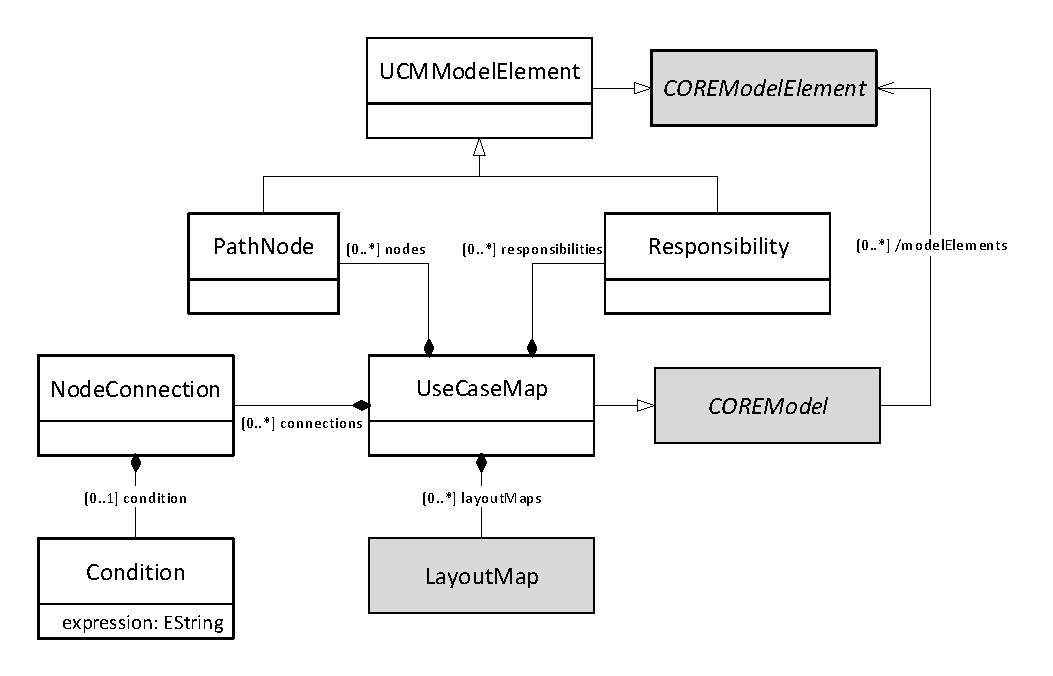
\includegraphics[scale=0.5]{fig_3_1.pdf}
	\caption{Extension of the CORE metamodel by UCM}
	\label{fig:3.1}
\end{figure}

We follow the URN specification~\cite{itu2012151} closely in corifying the UCM metamodel. Figure~\ref{fig:3.1} shows a partial view of the corified UCM metamodel, focusing on the elements that extend the CORE metamodel through subclassing (from an existing metaclass in the modeling language to an abstract CORE metaclass \footnote{The gray elements in the figures are the classes that derived from the CORE metamodel.}). By subclassing the necessary abstract classes of the CORE metamodel, UCM is able to provide all the properties of CORE:

\begin{enumerate}
	\setlength{\parskip}{0pt} \setlength{\itemsep}{0pt}
	\item A UCM model may now belong to a concern by realizing at least one of its features.
	\item A UCM realization model may now have impacts on high-level goals.
	\item A UCM model may extend another UCM model that belongs to a different feature.
	\item A UCM model may reuse another UCM model that belongs to a different concern.
\end{enumerate}

\todo[inline]{What follows is all about figuring out what the best customization interface for UCMs would be, and what the things are that will be mapped. I would introduce this maybe by presenting an example base scenario, and how one might want to extend it. Then show how one would model the example base scenario with a UCM, and then show how the extended UCM scenario would look like. Then explain how you envision to allow the modeller to not have to specify the complete extended scenario, but simply "augment" the base scenario with a model extension. Then proceed by explaining the details in the metamodel. If model reuse is very different from model extension then this should also be explained separately.}
The first and second properties are achieved once the UCM metamodel is properly extended, since CORE provides feature and goal modeling by default to all supported realization models. The third and forth properties, however, requires some thought on determining the customization interface that best suites UCMs, as customization interface is unique to all corified modeling languages and mappings should be tailored to each of the languages. After much deliberation, we arrived at a decision to provide mappings of different UCM model elements based on CORE model extensions and CORE model reuses.

Since the most common unit of occurrence for UCMs is responsibility that represents much of the actions in use cases, one of the most likely candidates for mapping is the responsibility element and is especially useful for model extensions. Aspect-oriented modeling can be carried out by combining separate UCM paths together, with mapped responsibilities act as join points. To illustrate the concept, %TODO

The idea of having a stub acts as a container for reusing UCM models is straightforward. Because the purpose of a stub is to bind plug-ins that consists of separate UCMs, a UCM model that is being reused can appear as a plug-in for the stub. Whereas the start and end points of the plug-ins connect the path segments coming in and going out of a stub to form the continuation of paths between the stub and plug-ins, similarly the start and end points of the reused UCM model connect the path segments coming in and going out of a stub. Reusing a UCM model is essentially reusing a concern---the selection of features when reusing a concern determines the final UCM model to be reused.

Reusing a concern from a UCM model prompts the feature selection process. This signals the feature that the UCM model realizes to reuse the other concern with the desired feature(s). The reusing UCM model then establishes the mappings to the reused UCM model that realizes the reused features. This is achieved as follows. The root element {\cls UseCaseMap} subclasses \textit{\cls COREModel}, which makes it part of a {\cls COREConcern} (see Figure~\ref{fig:2.1}, association between {\cls COREConcern} and {\cls COREModel}). This allows a UCM to realize a feature (see Figure~\ref{fig:2.2}, {\cls COREModel} realizes {\cls COREFeature}) within a concern. Therefore, the concern can create a {\cls COREReuse} to reuse another concern. The reusing UCM then creates a {\cls COREModelReuse} that has a direct association to the created {\cls COREReuse} and a \textit{\cls COREConfiguration} that selects the desired features from the reused concern. The CORE modeling tool then composes the UCM models of the reused concern that realize the selected features to generate a single woven user-tailored UCM model of the reused concern. Mappings to the model elements of this generated model are established using the class {\cls COREMapping}, consequently allowing the reusing UCM to customize the generated UCM model of the reused concern.

\begin{figure}
	\centering
	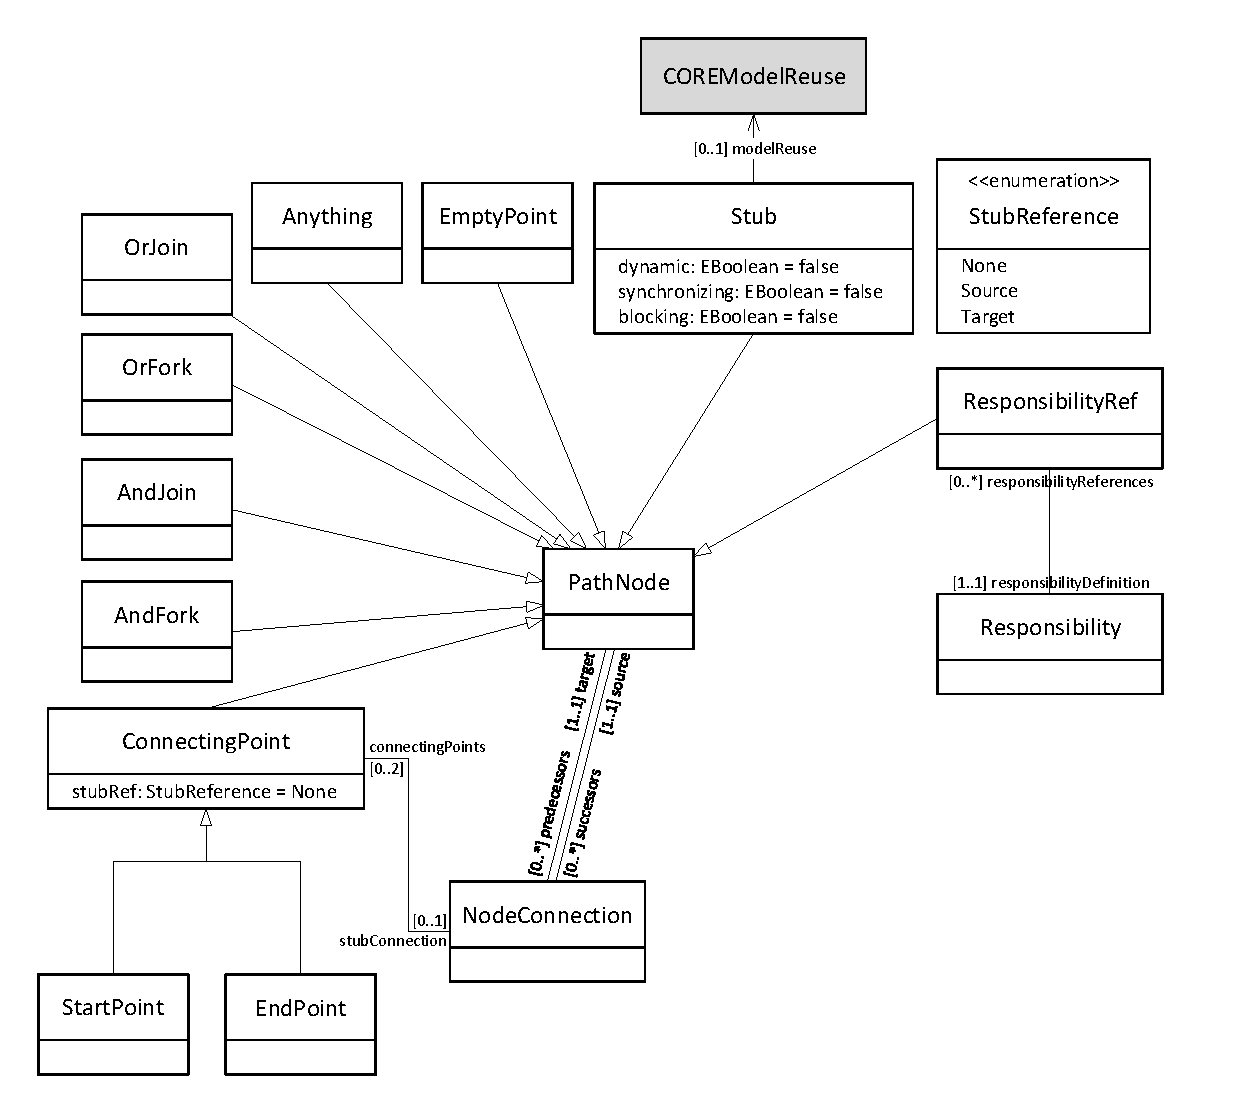
\includegraphics[scale=0.5]{fig_3_2.pdf}
	\caption{Path nodes for corified UCM}
	\label{fig:3.2}
\end{figure}

A standard UCM consists of {\cls PathNode}, {\cls Responsibility}, and {\cls NodeConnection}. {\cls LayoutMap} is added as part of the composition to allow positioning of the elements for viewing. We omit the inclusion of certain elements such as {\cls Component}, {\cls Timer}, and {\cls FailurePoint} to limit the scope of this thesis. On the contrary, {\cls PluginBinding} is excluded on purpose since we utilize {\cls COREMapping} as our approach to bind separate UCMs to {\cls Stub}. We incorporate several changes to the path nodes to support aspect-oriented modeling and reuse. Figure~\ref{fig:3.2} illustrates the addition of {\cls Anything} and {\cls ConnectingPoint}, as well as a directed association from {\cls Stub} to {\cls COREModelReuse}, to the UCM metamodel.

\textbf{\cls Anything:} We included the {\cls Anything} pointcut element from the extended AoUCM metamodel~\cite{mussbacher2011aspect}. {\cls Anything} acts as a wild card and can represent a subset of nodes in a path. This is useful for facilitating complex model weaving, as it allows any sequence of UCM model elements, including an empty sequence, to be matched.
\todo[inline]{Is this similar to the *-box in RAM that refers to the "original" behaviour of an advised sequence diagram? It might be interesting here to point out the similarities.}

\textbf{\cls ConnectingPoint:} We established a new path element to the metamodel. {\cls ConnectingPoint} is used to replace {\cls PluginBinding} and serves as an intermediate node that represents either a {\cls StartPoint} or an {\cls EndPoint}. By default, an actual start or end point within a UCM does not have a reference to a stub, hence the default value for {\cls StubReference} is {\cls None}. Instead, when we have a {\cls NodeConnection} that connects an element with a stub, then a hidden connecting point is automatically attached to the node connection (and deleted upon removal of the connection). Each node connection can have at most two connecting points if both the source and target nodes of the connection are stubs. Incoming connection to a stub generates a hidden end point with the value of {\cls stubRef} set to {\cls Target}, whereas outgoing connection from a stub generates a hidden start point with the value of {\cls stubRef} set to {\cls Source}. These hidden points allow us to define composition specifications through customization mappings.

\begin{figure}
	\centering
	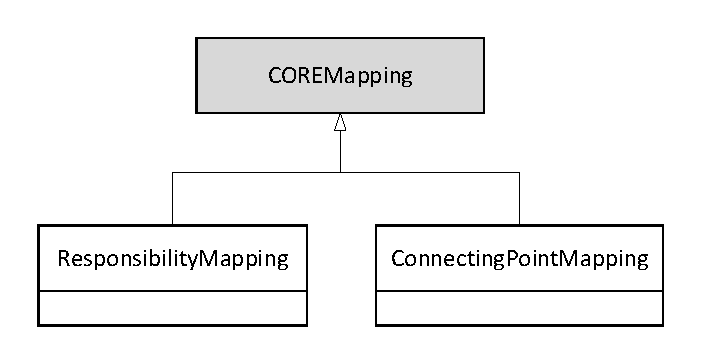
\includegraphics[scale=0.5]{fig_3_3.pdf}
	\caption{Customization mappings for corified UCM}
	\label{fig:3.3}
\end{figure}

Since we are using {\cls COREMapping} to specify customizations, it is necessary for {\cls UCMModelElement} to subclass \emph{\cls COREModelElement}. That way, all subclasses of {\cls UCMModelElement} (i.e., {\cls PathNode} and {\cls Responsibility}) can be used as source and destination classes for {\cls COREMapping}. As shown in Figure~\ref{fig:3.3}, we defined the composition specifications for specific UCM model elements: {\cls Responsibility} and {\cls ConnectingPoint}. They were selected so that we can compose UCM models based on the mappings of these elements. This leads us to the next section where we describe in detail how model composition is achieved through weaving.

\todo[inline]{I read up to here, but will continue soon}

\section{UCM Weaving} \label{sec:3.2}

As explained in Section~\ref{sec:2.1}, the role of the weaver is to facilitate model extensions and reuses. We offer two options when mapping elements between UCMs: (i) direct mapping of responsibilities; and (ii) cross mapping of connecting points. Cross mapping is necessary because of the nature of start and end points, where a start point of a UCM maps to an end point of a stub, and vice versa. A stub can be perceived as being superimposed with an end point followed by a start point, and those points collapsed into a point that is the stub \cite{buhr1995use}. Here, the hidden end point of a stub represents the incoming connection and it signifies the end of the sequence before the stub, and the hidden start point of a stub represents the outgoing connection and it signifies the start of the sequence after the stub. Both options have different procedures when weaving.

\subsection{Weaving Algorithm}

The algorithms presented here are specific for single weaving, meaning that a composition is performed from one model (\emph{UCM}\textsubscript{1}) to another model (\emph{UCM}\textsubscript{2}). This action can be chained together with other compositions, even with the hierarchical structure of the concern features. Here, we specify the subscript \textsubscript{1} for the model elements of a UCM the weaver composes from, and the subscript \textsubscript{2} for the model elements of a UCM the weaver composes to. \emph{UCM}\textsubscript{1} and \emph{UCM}\textsubscript{2} are merged prior to weaving, retaining all the path nodes and node connections from both models. Then the weaver iterates through the available composition specifications and executes the algorithms based on the specific type of mapping. The output of the woven model results in the amalgamation of UCMs based on the composition specification defined by the designer of the models, as well as the selected features of the concern by the user.

\subsubsection{Responsibility Mapping} \label{sec:3.2.1.1}

\begin{algorithm}
    \caption{Weaving Algorithm: Responsibility Mapping}
    \label{alg:1}
	\begin{algorithmic}[1]
	    \Function{WeaveResponsibilityMapping}{\emph{ucm}, \emph{composition}}
			\State \emph{node}\textsubscript{1} $\gets$ get first node of \emph{composition} mapping (\emph{from})
			\State \emph{node}\textsubscript{2} $\gets$ get second node of \emph{composition} mapping (\emph{to})
			\State mark \emph{node}\textsubscript{2} as visited
			\State indicate start point has not been encountered
			\State indicate end point has not been encountered
			\State call \Call{TraverseToSource}{\emph{ucm}, \emph{node}\textsubscript{2}, \emph{node}\textsubscript{1}}
			\State call \Call{TraverseToTarget}{\emph{ucm}, \emph{node}\textsubscript{2}, \emph{node}\textsubscript{1}}
			\State remove \emph{node}\textsubscript{1} from \emph{ucm}
		\EndFunction
		
		\Function{TraverseToSource}{\emph{ucm}, \emph{node}\textsubscript{2}, \emph{node}\textsubscript{1}}
			\For{each predecessor of \emph{node}\textsubscript{2}}
				\State \emph{sourceNode} $\gets$ get source node of predecessor
				\If{linkage exists from previous mapping} \label{alg:1.1}
					\State set the source of \emph{node}\textsubscript{2}'s connection to \emph{node}\textsubscript{1}'s predecessor
					\State disable linkage
					\State skip this loop
				\EndIf \label{alg:1.2}
				\If{\emph{sourceNode} is visited} \label{alg:1.3}
					\State skip this loop
				\ElsIf{\emph{sourceNode} is not {\cls Anything}}
					\State mark \emph{sourceNode} as visited
				\EndIf \label{alg:1.4}
				\If{\emph{sourceNode} is {\cls StartPoint} and start point is not encountered} \label{alg:1.5}
					\If{visibility of \emph{sourceNode} is {\cls Concern}}
						\State set the source of \emph{node}\textsubscript{2}'s connection to \emph{node}\textsubscript{1}'s predecessor
						\State remove \emph{sourceNode} from \emph{ucm}
						\State indicate start point has been encountered
					\EndIf \label{alg:1.6}
				\ElsIf{\emph{sourceNode} is {\cls Anything}} \label{alg:1.7}
					\State set the source of \emph{node}\textsubscript{2}'s connection to \emph{node}\textsubscript{1}'s predecessor
					\If{\emph{sourceNode} does not have any predecessor}
						\State remove \emph{sourceNode} from \emph{ucm}
					\EndIf \label{alg:1.8}
				\Else
					\State recursively call \Call{TraverseToSource}{\emph{ucm}, \emph{sourceNode}, \emph{node}\textsubscript{1}} \label{alg:1.9}
				\EndIf
			\EndFor
		\EndFunction
		
		\algstore{alg1}
	\end{algorithmic}
\end{algorithm}

\begin{algorithm}                     
	\begin{algorithmic}[1]
		\algrestore{alg1}
		
		\Function{TraverseToTarget}{\emph{ucm}, \emph{node}\textsubscript{2}, \emph{node}\textsubscript{1}}
			\For{each successor of \emph{node}\textsubscript{2}}
				\State \emph{targetNode} $\gets$ get target node of successor
				\If{\emph{targetNode} is visited} \label{alg:1.10}
					\State skip this loop
				\ElsIf{\emph{targetNode} is not {\cls Anything}}
					\State mark \emph{targetNode} as visited
				\EndIf \label{alg:1.11}
				\If{\emph{targetNode} is {\cls Endpoint} and end point is not encountered} \label{alg:1.12}
					\If{visibility of \emph{targetNode} is {\cls Concern}}
						\State set the target of \emph{node}\textsubscript{2}'s connection to \emph{node}\textsubscript{1}'s successor
						\State remove \emph{targetNode} from \emph{ucm}
						\State indicate end point has been encountered
					\EndIf \label{alg:1.13}
				\ElsIf{\emph{targetNode} is {\cls Anything}} \label{alg:1.14}
					\State set the target of \emph{node}\textsubscript{2}'s connection to \emph{node}\textsubscript{1}'s successor
					\If{\emph{targetNode} does not have any successor}
						\State remove \emph{targetNode} from \emph{ucm}
					\EndIf \label{alg:1.15}
				\ElsIf{\emph{targetNode} exists in \emph{composition} mapping (\emph{to})} \label{alg:1.16}
					\State copy node connection of successor
					\State set the target of copied connection to \emph{node}\textsubscript{1}'s successor
					\State add the copied connection to \emph{ucm}
					\State enable linkage to next mapping \label{alg:1.17}
				\Else
					\State recursively call \Call{TraverseToTarget}{\emph{ucm}, \emph{targetNode}, \emph{node}\textsubscript{1}} \label{alg:1.18}
				\EndIf
			\EndFor
		\EndFunction
	\end{algorithmic}
\end{algorithm}

Mapping with responsibilities allows for model extensions between parent and child UCMs. Composition specification can be defined by mapping from a parent UCM's responsibility to a child UCM's responsibility. Algorithm~\ref{alg:1} illustrates the procedure of weaving for responsibility mappings. The function \emph{WeaveResponsibilityMapping} initiates the process by identifying the mapped responsibilities (\emph{from} \emph{UCM}\textsubscript{1} \emph{to} \emph{UCM}\textsubscript{2}), and traversal begins from the point of \emph{responsibility}\textsubscript{2} in both directions: (i) toward predecessors until start point encountered; and (ii) toward successors until end point encountered. A UCM is represented as a directed graph, with possible cycles via {\cls OrFork}s and {\cls OrJoin}s. As such, we implemented a depth-first search approach for traversing the graph through recursion (lines~\ref{alg:1.9} and~\ref{alg:1.18}), and a mechanism to determine whether a node has been explored (lines~\ref{alg:1.3}-\ref{alg:1.4} and~\ref{alg:1.10}-\ref{alg:1.11}).

Furthermore, we allow multiple consecutive mappings between two UCM models. The path of a UCM may consist of mapped responsibilities interspersed with other path nodes. While traversing forward, lines~\ref{alg:1.16}-\ref{alg:1.17} handle the next mapped responsibility. If exist, forward traversal stops for this specific composition and appropriate nodes are connected between \emph{UCM}\textsubscript{1} and \emph{UCM}\textsubscript{2}. For subsequent mappings, lines~\ref{alg:1.1}-\ref{alg:1.2} handle the linkage from previous mappings, and backward traversal stops at the point of mapped responsibilities and appropriate nodes are connected between \emph{UCM}\textsubscript{1} and \emph{UCM}\textsubscript{2}. This pattern continues until the weaver reaches end point, whereby the predecessor of \emph{UCM}\textsubscript{2}'s end point connects to the successor of mapped responsibility (\emph{from}) \emph{UCM}\textsubscript{1} and this end point gets deleted (lines~\ref{alg:1.12}-\ref{alg:1.13}). Same goes for backward traversal until the weaver reaches start point (lines~\ref{alg:1.5}-\ref{alg:1.6}). Lastly, mapped responsibility (\emph{to}) \emph{UCM}\textsubscript{2} retains while mapped responsibility (\emph{from}) \emph{UCM}\textsubscript{1} gets deleted for the final woven UCM model.

UCM may have multiple start points merging to a path, or a path may branch to multiple end points. In this case, we allow a start or end point to set its visibility level. By default, connecting point is given the visibility of {\cls Concern} that signifies the start or end point is only visible when viewing a UCM model for a specific feature of a concern, but disappears after the composition process. The other option is {\cls Public} for global visibility and is used to retain the start or end point even after the composition process---the weaver would just ignore {\cls Public} connecting points and proceed to other branches. This feature is useful in defining multiple entry points, or alternative exit strategies, for a scenario.

Complex scenario model composition is also possible with the help of {\cls Anything}. An anything node can represent a subset of nodes in a path and is commonly used in \emph{UCM}\textsubscript{2} to capture the actual nodes that are specified in \emph{UCM}\textsubscript{1}. If an anything node is encountered during traversal, lines~\ref{alg:1.7}-\ref{alg:1.8} and~\ref{alg:1.14}-\ref{alg:1.15} signals the end of exploration and treat it as an end point. The difference is that the algorithm checks whether the anything node is still connected to other nodes before removal. This is necessary because an anything node has a predecessor node and a successor node, and typically surrounded by forks and joins (loop cycle). Both sides have to be traversed and dealt with before removing the anything node from the woven model.

\subsubsection{Connecting Point Mapping}

\begin{algorithm}
	\caption{Weaving Algorithm: Connecting Point Mapping}
	\label{alg:2}
	\begin{algorithmic}[1]
		\Function{WeaveConnectingPointMapping}{\emph{ucm}, \emph{composition}}
			\State \emph{node}\textsubscript{1} $\gets$ get first node of \emph{composition} mapping (\emph{from})
			\State \emph{node}\textsubscript{2} $\gets$ get second node of \emph{composition} mapping (\emph{to})
			\If{\emph{node}\textsubscript{1} is {\cls StartPoint}}
				\If{\emph{node}\textsubscript{1} is connected to a stub} \label{alg:2.1}
					\State call \Call{ExtendingStub\_End}{\emph{ucm}, \emph{node}\textsubscript{2}, \emph{node}\textsubscript{1}} \label{alg:2.2}
				\ElsIf{\emph{node}\textsubscript{2} is connected to a stub} \label{alg:2.3}
					\State call \Call{ReusingStub\_Start}{\emph{ucm}, \emph{node}\textsubscript{2}, \emph{node}\textsubscript{1}} \label{alg:2.4}
				\EndIf
			\ElsIf{\emph{node}\textsubscript{1} is {\cls EndPoint}}
				\If{\emph{node}\textsubscript{1} is connected to a stub} \label{alg:2.5}
					\State call \Call{ExtendingStub\_Start}{\emph{ucm}, \emph{node}\textsubscript{2}, \emph{node}\textsubscript{1}} \label{alg:2.6}
				\ElsIf{\emph{node}\textsubscript{2} is connected to a stub} \label{alg:2.7}
					\State call \Call{ReusingStub\_End}{\emph{ucm}, \emph{node}\textsubscript{2}, \emph{node}\textsubscript{1}} \label{alg:2.8}
				\EndIf
			\EndIf
		\EndFunction
		
		\Function{ExtendingStub\_End}{\emph{ucm}, \emph{node}\textsubscript{2}, \emph{node}\textsubscript{1}} \label{alg:2.9}
			\State \emph{source}\textsubscript{2} $\gets$ get source node of \emph{node}\textsubscript{2}
			\State \emph{source}\textsubscript{1} $\gets$ get source node of \emph{node}\textsubscript{1} via stub connection
			\State \emph{target}\textsubscript{1} $\gets$ get target node of \emph{node}\textsubscript{1} via stub connection
			\State call \Call{MergePaths}{\emph{source}\textsubscript{2}, \emph{source}\textsubscript{1}, \emph{target}\textsubscript{1}, \emph{node}\textsubscript{1}, \emph{node}\textsubscript{1}}
			\State remove \emph{node}\textsubscript{2} from \emph{ucm}
		\EndFunction \label{alg:2.10}
		
		\Function{ReusingStub\_Start}{\emph{ucm}, \emph{node}\textsubscript{2}, \emph{node}\textsubscript{1}} \label{alg:2.11}
			\State \emph{target}\textsubscript{1} $\gets$ get target node of \emph{node}\textsubscript{1}
			\State \emph{target}\textsubscript{2} $\gets$ get target node of \emph{node}\textsubscript{2} via stub connection
			\State \emph{source}\textsubscript{2} $\gets$ get source node of \emph{node}\textsubscript{2} via stub connection
			\State call \Call{SplitPaths}{\emph{target}\textsubscript{1}, \emph{target}\textsubscript{2}, \emph{source}\textsubscript{2}, \emph{node}\textsubscript{2}, \emph{node}\textsubscript{1}}
			\State remove \emph{node}\textsubscript{1} from \emph{ucm}
		\EndFunction \label{alg:2.12}
		
		\Function{ExtendingStub\_Start}{\emph{ucm} \emph{node}\textsubscript{2}, \emph{node}\textsubscript{1}} \label{alg:2.13}
			\State \emph{target}\textsubscript{2} $\gets$ get target node of \emph{node}\textsubscript{2}
			\State \emph{target}\textsubscript{1} $\gets$ get target node of \emph{node}\textsubscript{1} via stub connection
			\State \emph{source}\textsubscript{1} $\gets$ get source node of \emph{node}\textsubscript{1} via stub connection
			\State call \Call{SplitPaths}{\emph{target}\textsubscript{2}, \emph{target}\textsubscript{1}, \emph{source}\textsubscript{1}, \emph{node}\textsubscript{1}, \emph{node}\textsubscript{1}}
			\State remove \emph{node}\textsubscript{2} from \emph{ucm}
		\EndFunction \label{alg:2.14}
		
		\algstore{alg2}
	\end{algorithmic}
\end{algorithm}

\begin{algorithm}                     
	\begin{algorithmic}[1]
		\algrestore{alg2}
		
		\Function{ReusingStub\_End}{\emph{ucm}, \emph{node}\textsubscript{2}, \emph{node}\textsubscript{1}} \label{alg:2.15}
			\State \emph{source}\textsubscript{1} $\gets$ get source node of \emph{node}\textsubscript{1}
			\State \emph{source}\textsubscript{2} $\gets$ get source node of \emph{node}\textsubscript{2} via stub connection
			\State \emph{target}\textsubscript{2} $\gets$ get target node of \emph{node}\textsubscript{2} via stub connection
			\State call \Call{MergePaths}{\emph{source}\textsubscript{1}, \emph{source}\textsubscript{2}, \emph{target}\textsubscript{2}, \emph{node}\textsubscript{2}, \emph{node}\textsubscript{1}}
			\State remove \emph{node}\textsubscript{1} from \emph{ucm}
		\EndFunction \label{alg:2.16}
		
		\Function{SplitPaths}{\emph{target}, \emph{target}$'$, \emph{source}$'$, \emph{node}, \emph{node}$'$}
			\If{\emph{target}$'$ is {\cls Stub}} \label{alg:2.17}
				\State mark \emph{target}$'$ as removable stub
				\State set target node of \emph{node}'s stub connection to \emph{target} \label{alg:2.18}
			\ElsIf{\emph{target}$'$ is {\cls AndFork} or {\cls OrFork}} \label{alg:2.19}
				\State create node connection between \emph{target}$'$ and \emph{target} \label{alg:2.20}
			\Else \label{alg:2.21}
				\State \emph{referenceStub} $\gets$ get target node of \emph{node}$'$ via stub connection
				\State \emph{forkNode} $\gets$ \textbf{if} \emph{referenceStub} is dynamic \textbf{then} create {\cls AndFork} \textbf{else} {\cls OrFork}
				\State place \emph{forkNode} in between \emph{source}$'$ and \emph{target}$'$
				\State create node connection between \emph{forkNode} and \emph{target}$'$
				\State create node connection between \emph{forkNode} and \emph{target}
				\State set target node of \emph{node}'s stub connection to \emph{forkNode}
			\EndIf \label{alg:2.22}
		\EndFunction
		
		\Function{MergePaths}{\emph{source}, \emph{source}$'$, \emph{target}$'$, \emph{node}, \emph{node}$'$}
			\If{\emph{source}$'$ is {\cls Stub}} \label{alg:2.23}
				\State mark \emph{source}$'$ as removable stub
				\State set source node of \emph{node}'s stub connection to \emph{source} \label{alg:2.24}
			\ElsIf{\emph{source}$'$ is {\cls AndJoin} or {\cls OrJoin}} \label{alg:2.25}
				\State create node connection between \emph{source} and \emph{source}$'$ \label{alg:2.26}
			\Else \label{alg:2.27}
				\State \emph{referenceStub} $\gets$ get source node of \emph{node}$'$ via stub connection
				\State \emph{joinNode} $\gets$ \textbf{if} \emph{referenceStub} is synchronizing \textbf{then} create {\cls AndJoin} \textbf{else} {\cls OrJoin}
				\State place \emph{joinNode} in between \emph{source}$'$ and \emph{target}$'$
				\State create node connection between \emph{source}$'$ and \emph{joinNode}
				\State create node connection between \emph{source} and \emph{joinNode}
				\State set source node of \emph{node}'s stub connection to \emph{joinNode}
			\EndIf \label{alg:2.28}
		\EndFunction
	\end{algorithmic}
\end{algorithm}

Mapping with connecting points allows for model extensions between parent and child UCMs and also model reuses from UCMs of other concerns. Algorithm~\ref{alg:2} illustrates the procedure of weaving for connecting point mappings. The function \emph{WeaveConnectingPointMapping} initiates the process by identifying the mapped connecting points (\emph{from} \emph{UCM}\textsubscript{1} \emph{to} \emph{UCM}\textsubscript{2}), and determine the type of composition to be performed based on whether the connecting points mapped from \emph{UCM}\textsubscript{1} are attached to a stub or not. If the mapped start and end points from \emph{UCM}\textsubscript{1} are attached to a stub (lines~\ref{alg:2.1}-\ref{alg:2.2} and~\ref{alg:2.5}-\ref{alg:2.6}), it means that the connecting points are hidden and belong to a stub in \emph{UCM}\textsubscript{1} and are mapped to actual end and start points of \emph{UCM}\textsubscript{2}, respectively (cross mapping). This type of composition is model extension. Vice versa for model reuse (lines~\ref{alg:2.3}-\ref{alg:2.4} and~\ref{alg:2.7}-\ref{alg:2.8}).

Model extension for stubs work differently compared with responsibilities. No traversal is required since there is no need to explore the whole graph, but the composition specification requires exactly two connecting point mappings for each stub to be complete---one for the start point and the second for end point. The weaver first obtain the pair of mappings for the stub. The initial mapping usually maps the end point of a stub \footnote{The end point of a stub symbolizes incoming node connection to the stub.} to the start point of a UCM, and the weaver executes lines~\ref{alg:2.9}-\ref{alg:2.10}. The second mapping usually maps the start point of a stub \footnote{The start point of a stub symbolizes outgoing node connection from the stub.} to the end point of a UCM, and the weaver executes lines~\ref{alg:2.13}-\ref{alg:2.14}.

Model reuse, on the other hand, operates in reversed orientation---obtaining the pairs of mappings that mapped the start and end points of \emph{UCM}\textsubscript{1} to the connecting points of a stub that is automatically generated in \emph{UCM}\textsubscript{2} when reusing \emph{UCM}\textsubscript{1}. To be precise, the automatically generated stub is always a static stub so that it can only hold a single UCM that originates from the reused concern. The weaver then executes lines~\ref{alg:2.11}-\ref{alg:2.12} and~\ref{alg:2.15}-\ref{alg:2.16}, respectively.

The execution procedure for both extension and reuse involves replacing a stub with plug-ins (sub-UCMs). Depending on the type of stub, it can bind either a single plug-in or multiple plug-ins. When facing a single plug-in bound to a stub, the weaver simply connects the nodes adjacent to the stub and nodes adjacent to the connecting points of a UCM, followed by the removal of the connecting points and the stub from the woven model (lines~\ref{alg:2.17}-\ref{alg:2.18} and~\ref{alg:2.23}-\ref{alg:2.24}). If there are two plug-ins bound to a stub, the weaver creates branches to link the two UCMs as parallel paths via fork and join nodes (lines~\ref{alg:2.21}-\ref{alg:2.22} and~\ref{alg:2.27}-\ref{alg:2.28}). The type of forks and joins being created is dependent on the type of stub. Synchronizing/blocking stubs produce branches that consist of {\cls AndFork} and {\cls AndJoin}, dynamic stubs produce branches that consist of {\cls AndFork} and {\cls OrJoin}, and static stubs produce branches that consist of {\cls OrFork} and {\cls OrJoin}. This process is also known as semantic flattening \cite{itu2012151}. Additional plug-ins bound to a stub are linked via the created forks and joins (lines~\ref{alg:2.19}-\ref{alg:2.20} and~\ref{alg:2.25}-\ref{alg:2.26}).


\chapter{Validation} \label{ch:4}
The definition of UCM metamodel and the specification of weaving algorithm described in the previous chapter provide the foundation for the implementation of UCM in TouchCORE, a multitouch-enabled concern-oriented software design modeling tool. In this chapter, we illustrate the realization of scenario models in TouchCORE through the use of UCM notation in section~\ref{sec:4.1}. Then we attempt to validate our proposed approach of concern-oriented UCMs by means of case studies in section~\ref{sec:4.2}. Finally, we demonstrate that concern-oriented UCMs are able to cover the workflow patterns in section~\ref{sec:4.3}.

\section{UCM Implementation in TouchCORE} \label{sec:4.1}

TouchCORE is under active development within the Software Engineering Lab at McGill University \cite{sel2015touchcore}. Previous project, TouchRAM, successfully implemented concern-oriented software design paradigm, but support is limited to RAM (class, sequence, and state diagrams) \cite{al2012touchram, schottle2014touchram}. TouchCORE extends TouchRAM with numerous enhancements, most notably the support for arbitrary modeling languages in addition to RAM. Since we have a well-defined corified UCM metamodel, we attempted to add support for UCMs in TouchCORE as proof of concept, enabling TouchCORE the capability to build scalable and reusable scenario models.

The project uses Java SE Development Kit 8 as the implementation language and Eclipse Modeling Framework (EMF)~\cite{steinberg2008emf} as the modeling facility for developing TouchCORE. To support a new language, we need to define its metamodel based on Ecore. TouchCORE already has a complete CORE metamodel defined with an Ecore model (see Figure~\ref{fig:a.1}). With RAM as a reference model, we constructed an Ecore model that expresses our complete UCM metamodel, subclassing the appropriate CORE metaclasses, through the use of EMF tooling (see Figure~\ref{fig:a.2} in Appendix~\ref{ch:A} for complete UCM metamodel). EMF is capable of generating structured Java code from valid Ecore models, allowing us to rapidly program the logic for UCM integration.

\begin{figure}
	\centering
	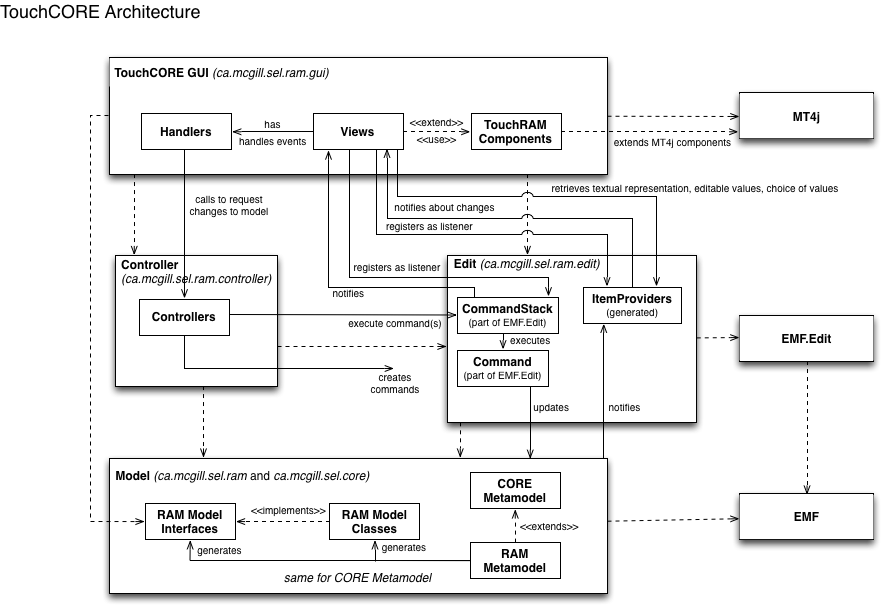
\includegraphics[scale=0.5]{fig_4_1.png}
	\caption[TouchCORE architecture]{TouchCORE architecture. Image courtesy of Software Engineering Lab, McGill University}
	\label{fig:4.1}
\end{figure}

The software architecture of TouchCORE follows the model–view–controller (MVC) design pattern to separate the program into three main logical components. Figure~\ref{fig:4.1} shows the three interconnected parts for the TouchCORE application: (i) the model layer for managing data, e.g., instances of RAM and UCM models; (ii) the TouchCORE graphical user interface (GUI) that constitutes the view layer for visualizing and manipulating models; and (iii) the controller layer for handling user interactions and act on the data model objects. The GUI for TouchCORE is built on top of MT4j for its multitouch capability \cite{laufs2010mt4j}. Additional components include weaver, code generator, model validator, and classloader. The integration of UCM in TouchCORE involves modifying its core components with varying degrees, but the program is structured in such a way that we can add subcomponents when implementing a new modeling language, adhering to the open/closed principle.

\subsection{Supported Concrete Syntax}

\begin{figure}[h]
	\centering
	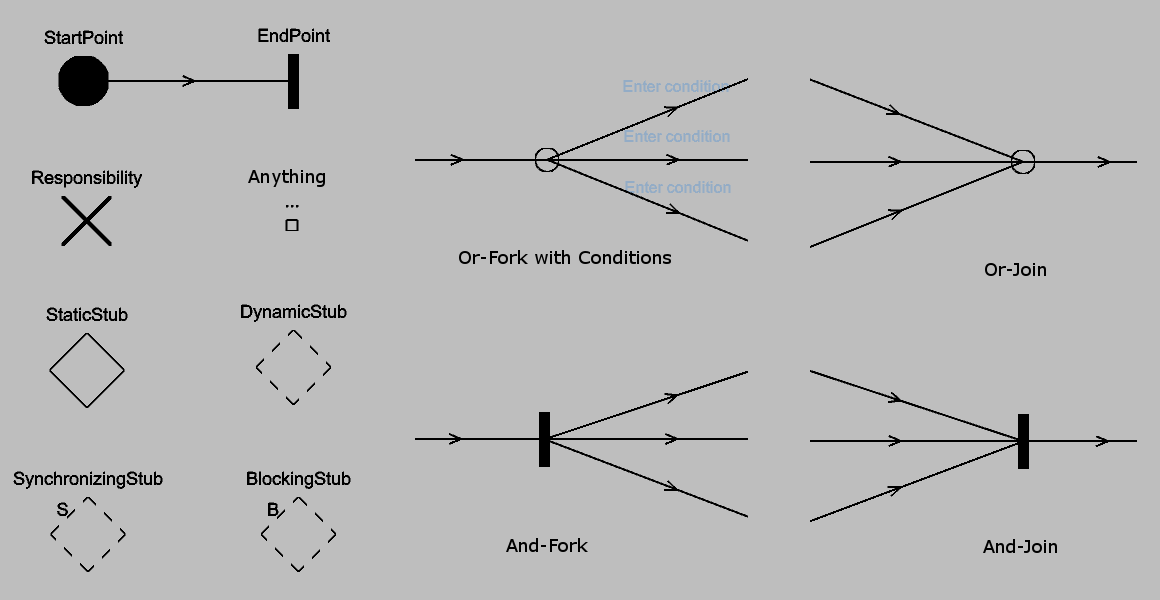
\includegraphics[scale=0.3]{fig_4_2.png}
	\caption{UCM notation in TouchCORE}
	\label{fig:4.2}
\end{figure}

The basic elements of the UCM notation that we implemented in TouchCORE are shown in Figure~\ref{fig:4.2}. Most of these elements are defined by the standards~\cite{itu2012151}, with the exception of {\cls Anything} that is taken from the extended AoUCM metamodel~\cite{mussbacher2011aspect}. Users can create path nodes by tap-and-hold on the canvas of TouchCORE during runtime and a list of path nodes will be displayed for selection. To create a node connection between two path nodes, simply drag from the area adjacent of one element to the other element.

There are several anomalies with regards to the graphical representation of UCM symbols displayed in TouchCORE as compared with the standards (compare Figure~\ref{fig:4.2} with Figure~\ref{fig:2.7}). For example, the symbol for OR-fork and OR-join is shown as a circle instead of no symbol (just direct branching and merging from the paths); anything is represented as a square with the label \ldots\ instead of just \ldots; and node connection is a straight line path instead of spline. These are some of the limitations that we faced at the moment when implementing the GUI. Our current method of creating nodes is to first create them on the canvas, then build the connections later. OR-fork and OR-join need a space to receive events from the user, thus a circle serves as the area of interactivity as well as a statement of presence that an OR-fork or OR-join has been created. The idea of displaying the \ldots symbol of an anything node is that it should be part of the node connection and move along seamlessly with correct orientation whenever the predecessor or successor node of anything is moved, but since anything is considered a path node, we decided for now to just use a square with the label \ldots\ to represent the anything node. Lastly, spline drawing is not yet available in TouchCORE so we use straight lines for the time being.

\begin{figure}
	\centering
	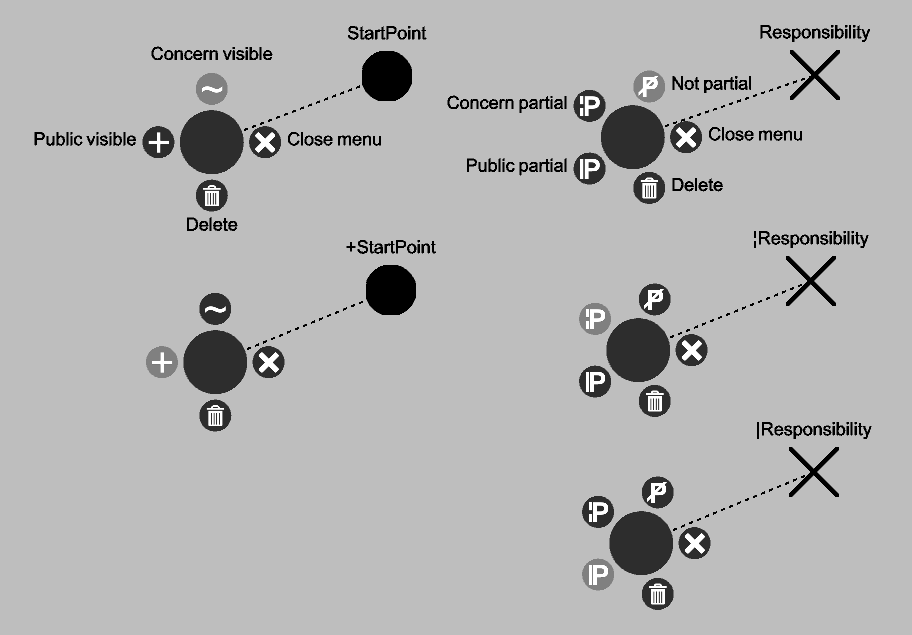
\includegraphics[scale=0.3]{fig_4_3.png}
	\caption{Visibility and partiality}
	\label{fig:4.3}
\end{figure}

Elements with extra features can be accessed by tap-and-hold an element (Figure~\ref{fig:4.3}). We allow start and end points to set its visibility. By default, all path nodes are concern visible, but start and end points can switch to public visible (see Section~\ref{sec:3.2.1.1} for visibility discussion). Likewise, we allow responsibilities to set its partiality. By default, all path nodes are not partial, meaning they are well-defined and require no further action. Since we have customization mappings for responsibility, we can specify whether a responsibility is partially defined and require appropriate composition to be semantically complete. A responsibility that is concern partial should fulfill its significance through model extension, whereas a responsibility that is public partial should fulfill its significance through model reuse.

\subsection{Scenario Model Composition}

\subsubsection{Model Extension}

\begin{figure}
	\centering
	\subfloat[Model A - parent UCM]{\label{fig:4.4a}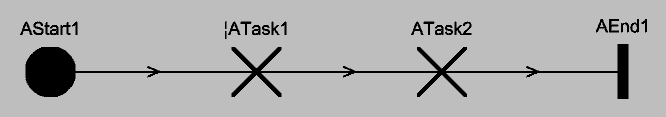
\includegraphics[clip,width=0.7\columnwidth]{fig_4_4a.png}} \\
	\subfloat[Model B - child UCM]{\label{fig:4.4b}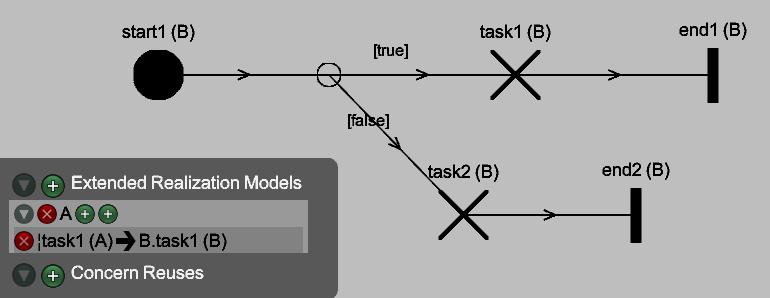
\includegraphics[clip,width=0.7\columnwidth]{fig_4_4b.png}} \\
	\subfloat[Woven Model B\_A]{\label{fig:4.4c}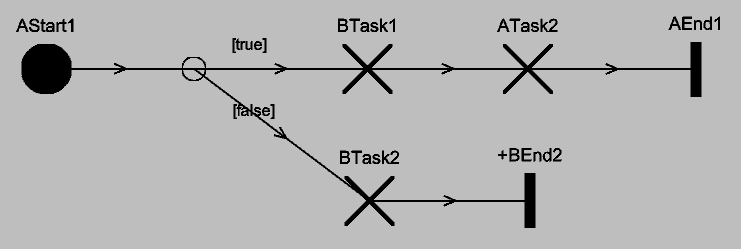
\includegraphics[clip,width=0.7\columnwidth]{fig_4_4c.png}}
	\caption{Schematic representation of model extension}
	\label{fig:4.4}
\end{figure}

Figure~\ref{fig:4.4} illustrates the usage of UCM model extension within a concern. Given a concern with two features in a hierarchy, the model of a child feature (Model B) extends the model of a parent feature (Model A). Composition specifications are specified in Model B, where an element of Model A is mapped to an element of Model B. Multiple mappings can be set per extension as needed and the available types of mapping are defined in the metamodel. The result of weaving Model B to Model A is depicted in Figure~\ref{fig:4.4c}. Based on the mappings set in Model B, the predecessors and successors of the mapped responsibility from Model B are introduced as adjoined path nodes of the mapped responsibility from Model A, and the mapped responsibility from Model A is being replaced with the mapped responsibility from Model B.

The idea of isolating features as individual models supports the use of advanced separation of concerns---each feature encapsulates its realization model. Features of a concern are nested in a hierarchical order, and the connection between features can be seen as parent-child relationship. Extension of a model depends on this relationship to ensure that models are woven in the correct order. Only the selected features of a concern are woven as a whole, providing only the absolute necessary details to fully describe the different use cases.

\subsubsection{Model Reuse}

\begin{figure}
	\centering
	\subfloat[Model C - reuse Concern A with selected features <A,B>]{\label{fig:4.5a}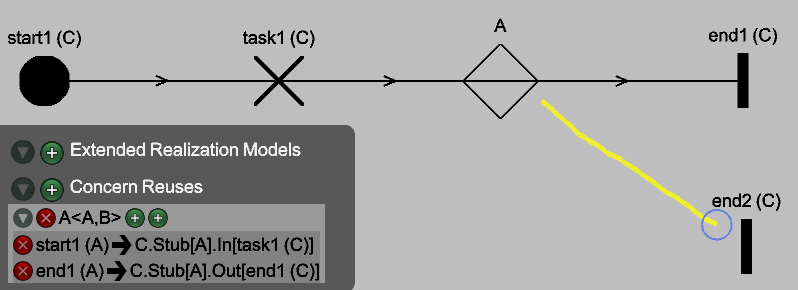
\includegraphics[clip,width=0.7\columnwidth]{fig_4_5a.png}} \\
	\subfloat[Model C - establish connecting point mapping through node connection]{\label{fig:4.5b}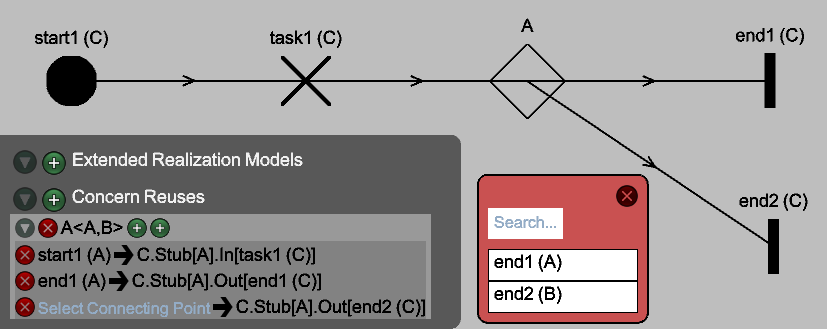
\includegraphics[clip,width=0.7\columnwidth]{fig_4_5b.png}} \\
	\subfloat[Woven Model C\_A<A,B>]{\label{fig:4.5c}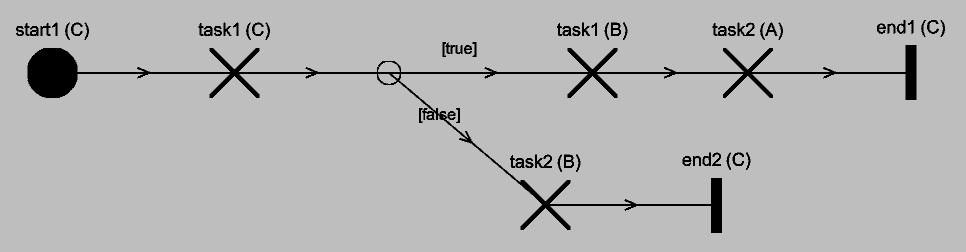
\includegraphics[clip,width=0.7\columnwidth]{fig_4_5c.png}}
	\caption{Schematic representation of model reuse}
	\label{fig:4.5}
\end{figure}

Figure~\ref{fig:4.5} illustrates the usage of UCM model reuse across concerns. Given that Model C of a concern reuses Concern A, the configuration for the set of features of Concern A will be displayed. Here, we chose to use features A and B, thus woven Model B\_A (see Figure~\ref{fig:4.4c}) is generated and represented as a static Stub A (appears automatically in canvas after successful reuse). Mappings for connecting points of Stub A can be established by linking a path node to/from Stub A. As shown in Figures~\ref{fig:4.5a} and~\ref{fig:4.5b}, a node connection was created from Stub A to an end point, and a list of end points from woven Model B\_A will be displayed for the user to set which end point of Model B\_A corresponds to which outgoing connection of Stub A in Model C. We label the incoming connection of a stub as \verb|<Model_2>.Stub[<Model_1>].In[<Predecessor>]|, and the outgoing connection as \verb|<Model_2>.Stub[<Model_1>].Out[<Successor>]|. The result of weaving Model C to Model B\_A is depicted in Figure~\ref{fig:4.5c}.

\section{Case Studies} \label{sec:4.2}

In this section, we attempt to validate our proposed technique for concern-oriented UCMs with two case studies: Authentication and Online Payment. We chose these two examples as our case studies because they provide different yet appropriate level of complexity to the problem that we are studying, as well as the ability to reuse the Authentication concern within the Online Payment concern.

\subsection{Authentication}

\begin{figure}[h]
	\centering
	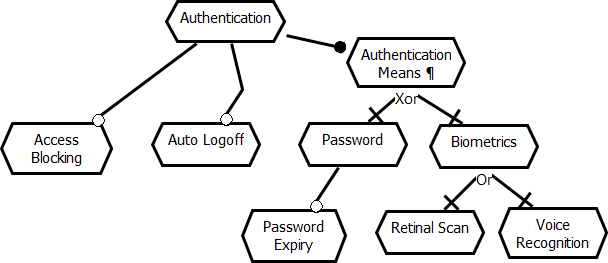
\includegraphics[scale=0.5]{fig_4_6.png}
	\caption[Feature model for Authentication (jUCMNav)]{Feature model for Authentication (jUCMNav). Image courtesy of Nishanth Thimmegowda et al.~\cite{thimmegowda2014concern}}
	\label{fig:4.6}
\end{figure}

We design the Authentication concern based on a reference model that we have previously described in jUCMNav format~\cite{thimmegowda2014concern}. Figure~\ref{fig:4.6} shows all the available features that are supported for the concern. \emph{Authentication} has a mandatory \emph{Authentication Means} feature that may either be \emph{Password} that can be extended with the optional \emph{Password Expiry} feature, or \emph{Biometrics} that requires at least \emph{Retinal Scan} or \emph{Voice Recognition}. If necessary, consecutive unsuccessful authentication attempts may result in \emph{Access Blocking} and long idle period may lead to \emph{Auto Logoff}.

\begin{figure}
	\centering
	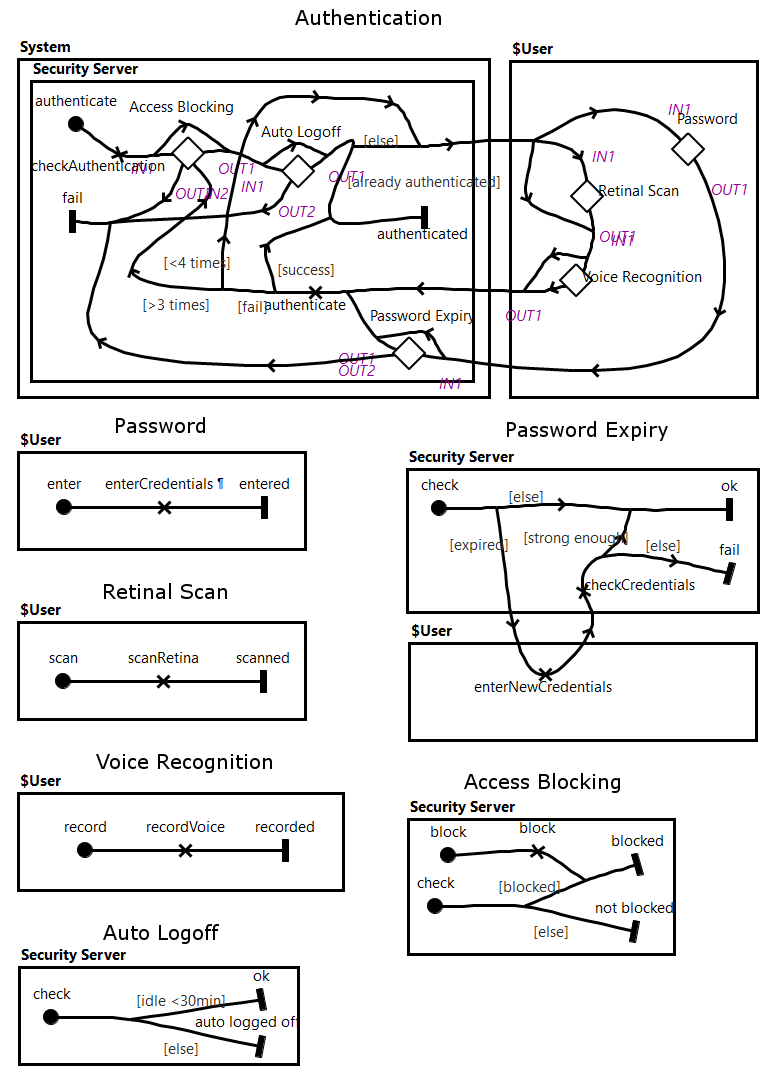
\includegraphics[scale=2]{fig_4_7.png}
	\caption[Scenario models for Authentication (jUCMNav)]{Scenario models for Authentication (jUCMNav). Image courtesy of Nishanth Thimmegowda et al.~\cite{thimmegowda2014concern}}
	\label{fig:4.7}
\end{figure}

\begin{figure}
	\centering
	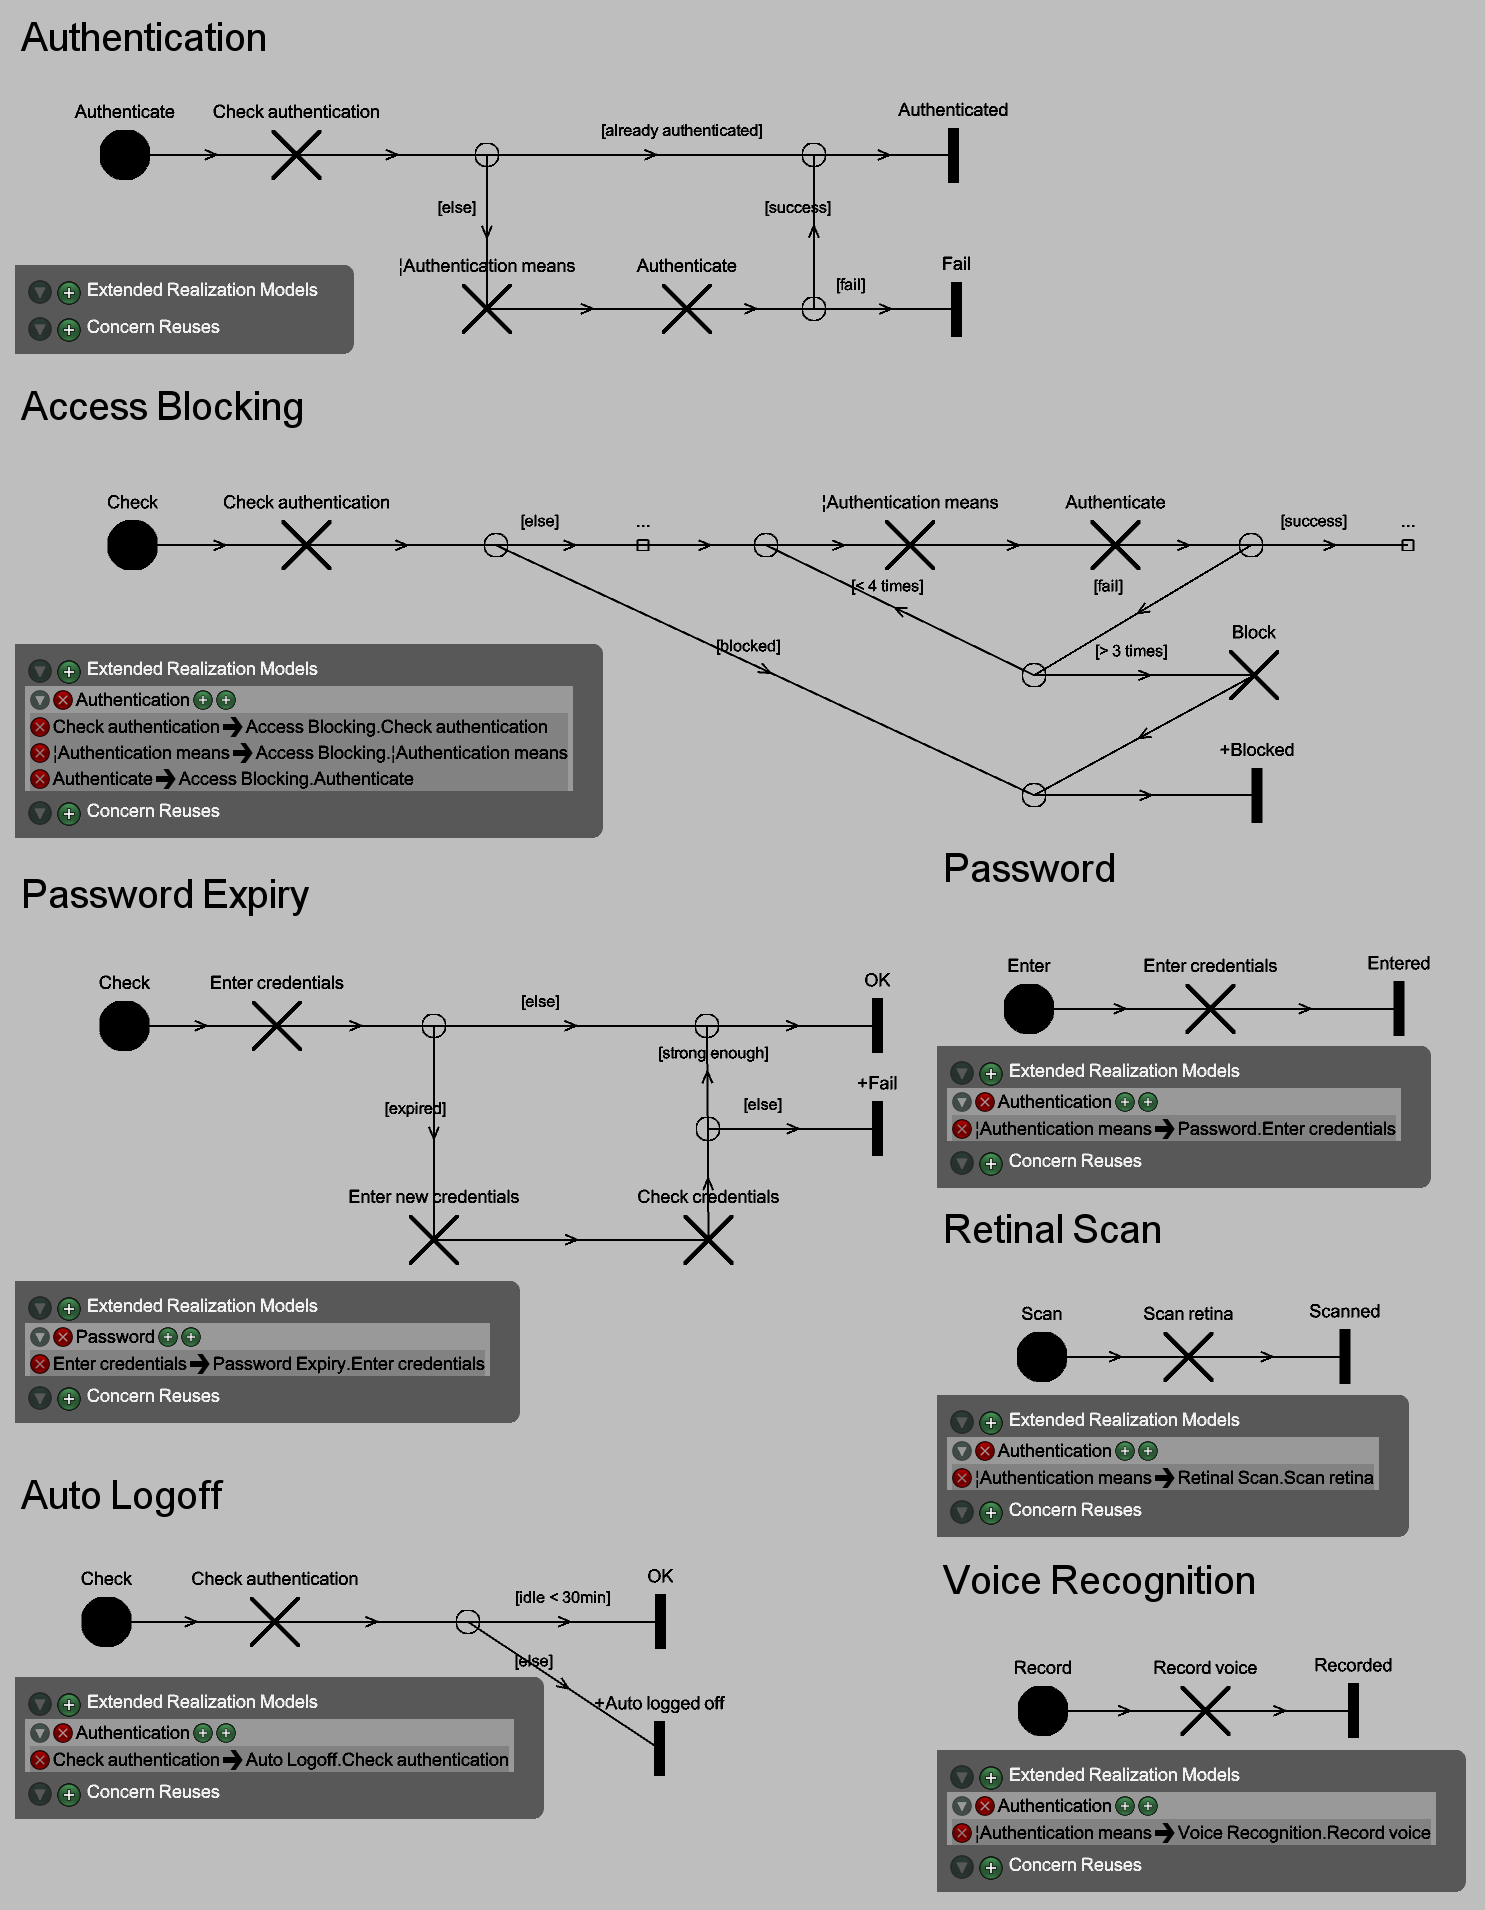
\includegraphics[scale=1.2]{fig_4_8.png}
	\caption{Scenario models for Authentication (TouchCORE)}
	\label{fig:4.8}
\end{figure}

Scenario models can be (optionally) realized for the features to describe how the user would interact with the Authentication concern. Figure~\ref{fig:4.7} illustrates the UCM diagrams and plug-ins that are realized for most of the features. Then, with slight modifications to the UCMs specified in jUCMNav, we developed our version of the UCMs using TouchCORE as depicted in Figure~\ref{fig:4.8}. (Feature model remains unchanged and TouchCORE version of the feature model is omitted.)

Notice that in the root map of Figure~\ref{fig:4.7}, each feature is represented as a static stub and is bound to a plug-in for the feature. In the root map developed using TouchCORE (see Figure~\ref{fig:4.8}), we minimize the usage of stubs and instead utilize model extensions, successfully isolating the aspects of crosscutting the core concern. Since \emph{Authentication Means} is a mandatory feature, we introduce a responsibility placeholder and set its partiality to concern partial. Any UCMs under the \emph{Authentication Means} feature can extend the root UCM via responsibility mapping. One advantage of using CORE approach in modeling UCMs is that by selecting the desired features when reusing this concern, only the UCMs of those selected features will be composed into the root map and a single UCM that consists of only the necessary paths will be generated. The woven UCM can be reused in another concern such as Online Payment.

\subsection{Online Payment}

\begin{figure}[h]
	\centering
	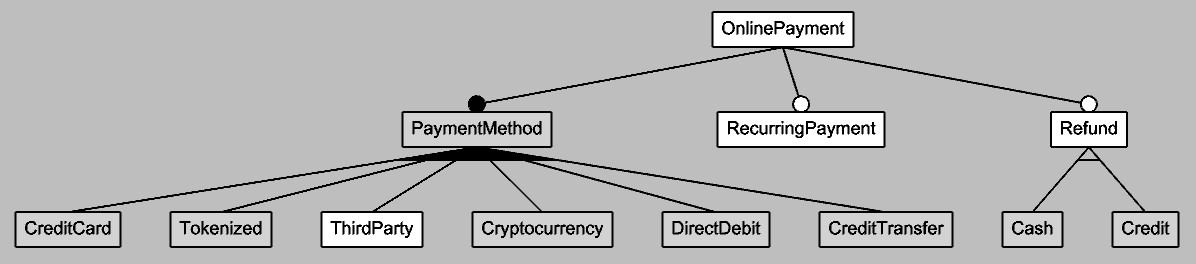
\includegraphics[scale=1.5]{fig_4_9.png}
	\caption{Feature model for Online Payment}
	\label{fig:4.9}
\end{figure}

\begin{figure}
	\centering
	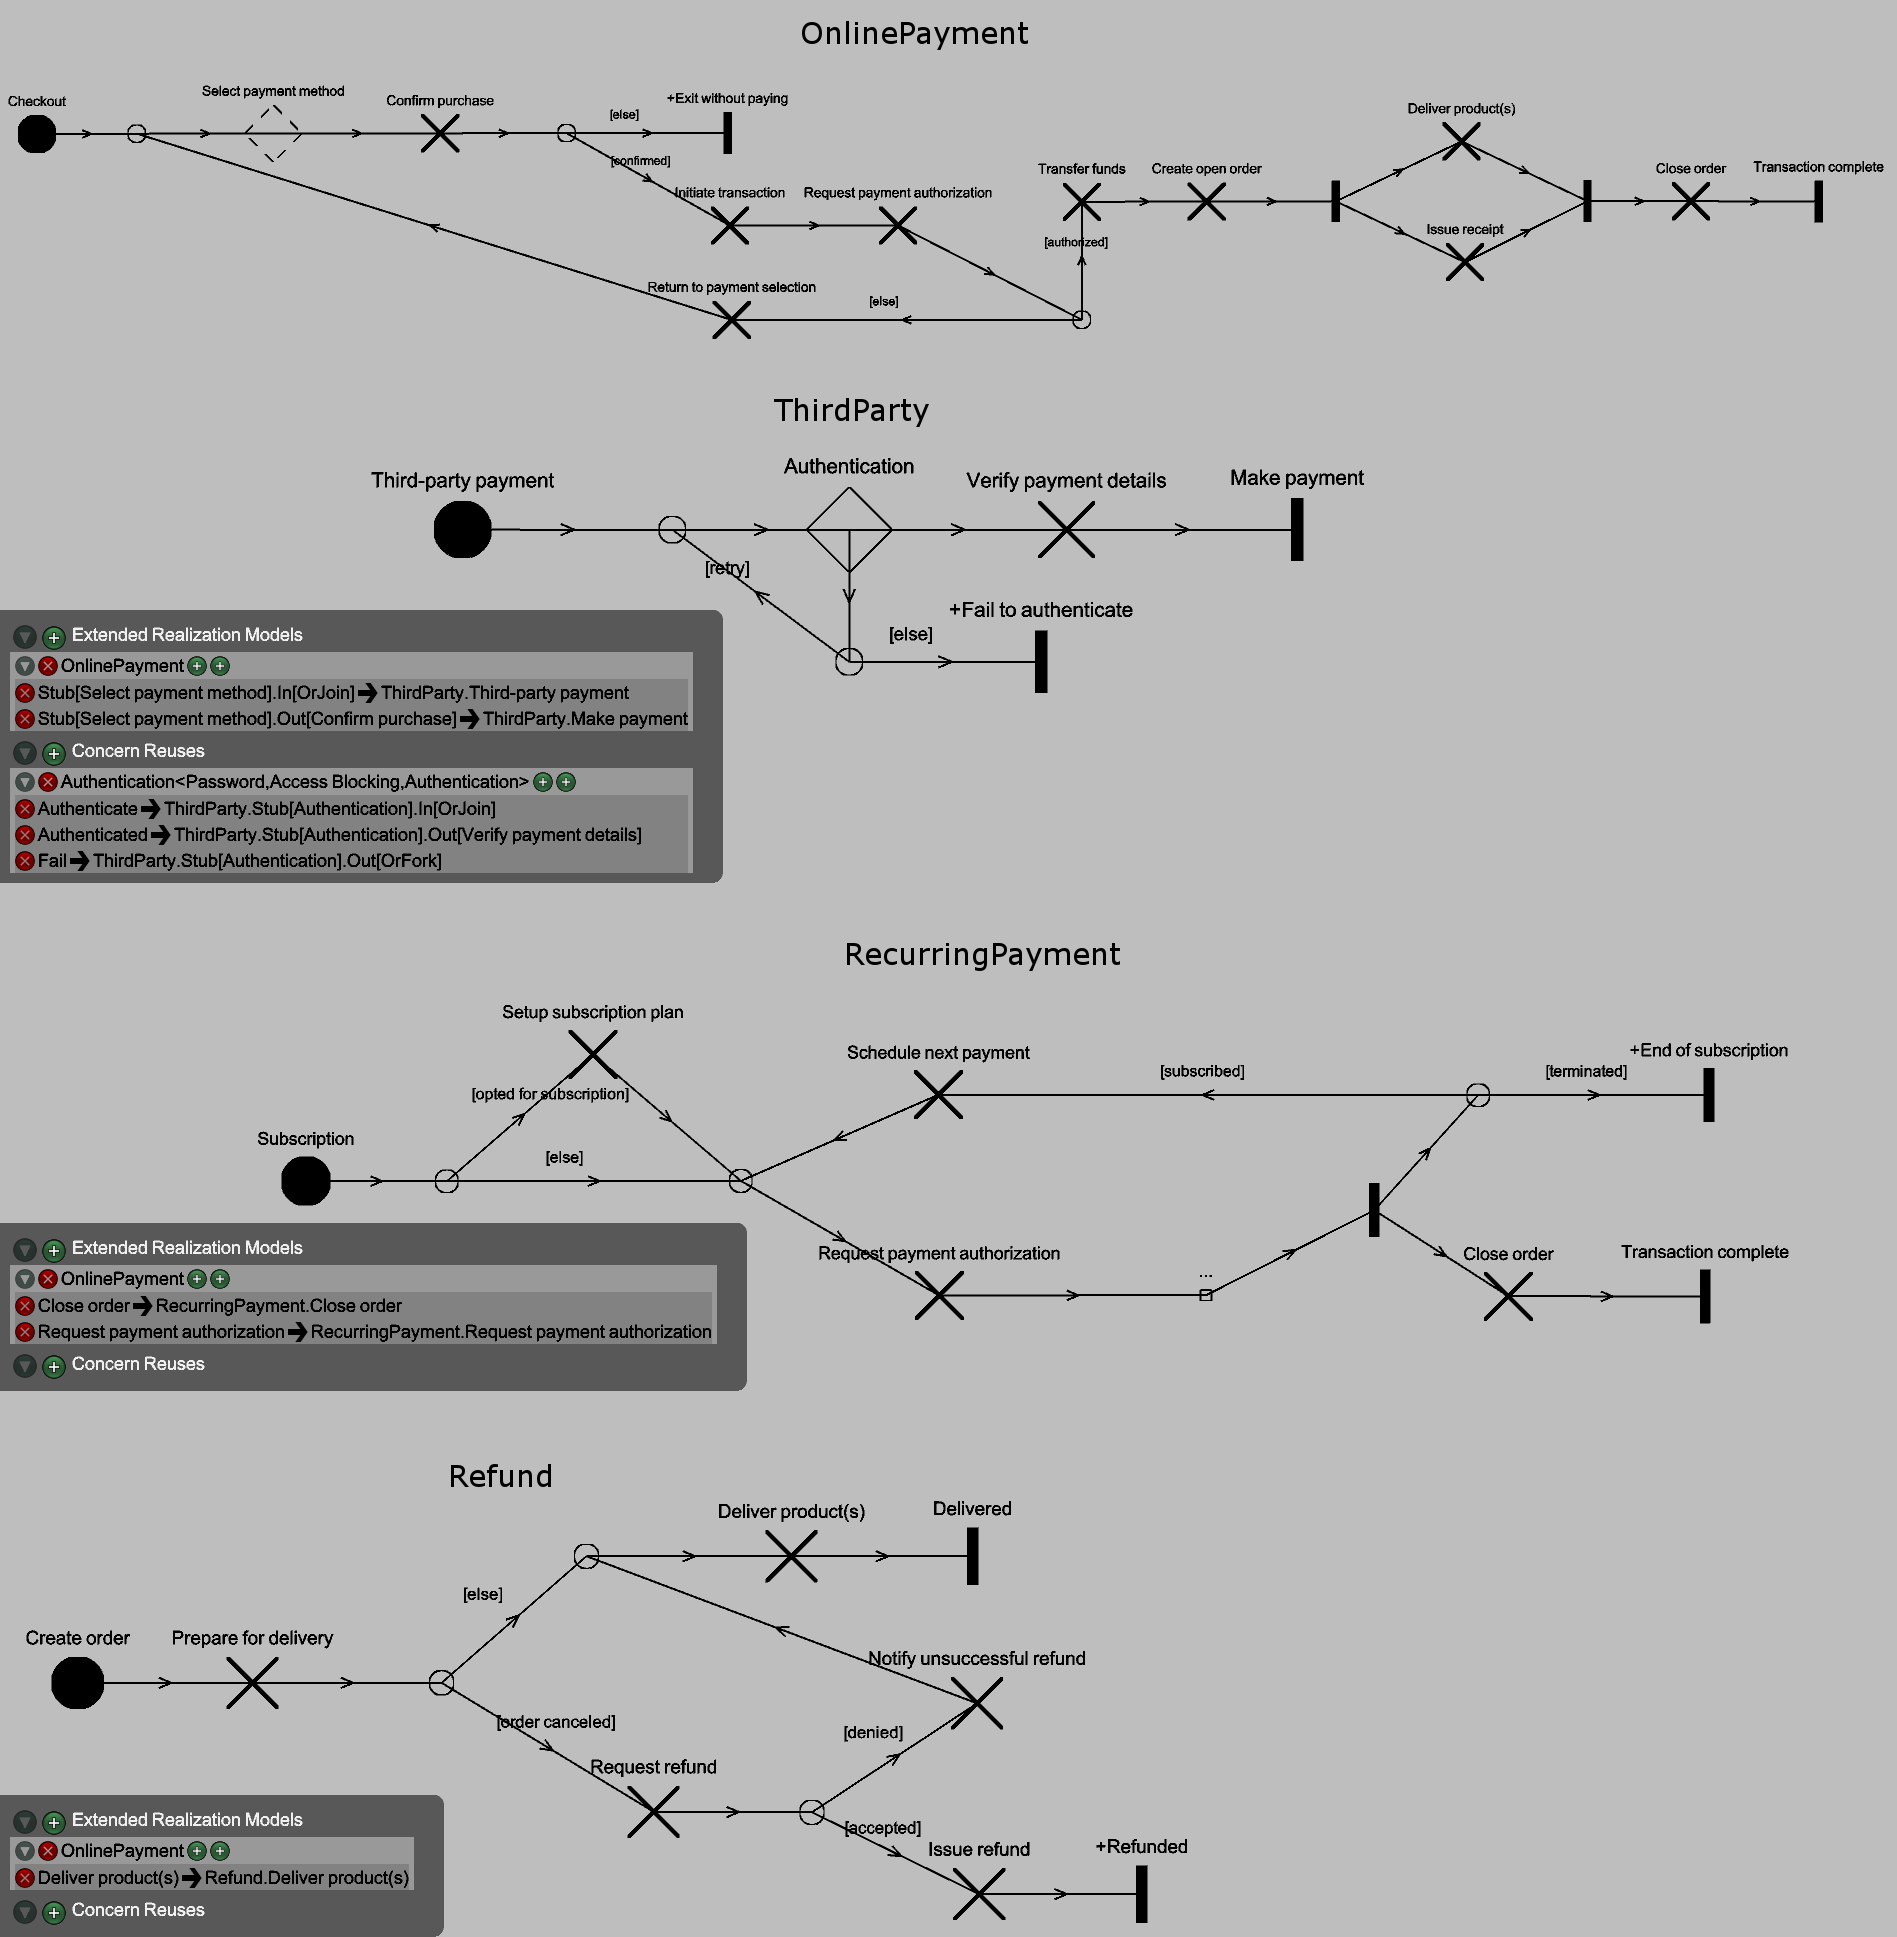
\includegraphics[scale=1]{fig_4_10.png}
	\caption{Scenario models for Online Payment}
	\label{fig:4.10}
\end{figure}

The Online Payment concern offers a means to build a payment model for e-commerce platform. Use cases for Online Payment are adapted from W3C Web Payments Interest Group \cite{w3c2015web}, focusing on the payment schemes in use today. Figure~\ref{fig:4.9} shows all the available features that are supported for the concern. Online Payment provides numerous payment methods for the customers to pay by credit card (e.g., Visa, MasterCard, China UnionPay), tokenized payment (e.g., ApplePay, Venmo, CyberSource), third-party payment (e.g., PayPal, Alipay, Google Pay), cryptocurrency (e.g., Bitcoin, Ripple, Ethereum), direct debit, or credit transfer. Optionally, the system supports recurring payment option to allow for subscription plan and refund to the payer's payment instrument or store credit.

Figure~\ref{fig:4.10} illustrates a typical workflow for Online Payment. In the root map, we have a single entry and exit point---from checkout to transaction complete---and a loop that redirects the user back to the payment selection if payment authorization fails. The payment method selection is modeled as a dynamic stub to receive multiple plug-ins from the subfeatures of \emph{PaymentMethod}. We limit the discussion of \emph{PaymentMethod} to \emph{ThirdParty} since the scenario model for paying through third-party is sufficient to describe the essential features and most methods share similar scenario. There are two things worth mentioning in the \emph{ThirdParty} model. First, \emph{ThirdParty} extends \emph{OnlinePayment} through the \emph{Select payment method} dynamic stub, hence mapping is done via connecting points. Second, \emph{ThirdParty} reuses the Authentication concern is depicted as a static stub, and the selected features are \emph{Password} and \emph{Access Blocking}. The one incoming connection and two outgoing connections of the \emph{Authentication} stub are associated with the single start point (\emph{Authenticate}) and two end points (\emph{Authenticated}; \emph{Fail}) of Authentication UCM (see Figure~\ref{fig:4.8}).

Optional features of \emph{OnlinePayment} are \emph{RecurringPayment} and \emph{Refund}. Both of the features extend \emph{OnlinePayment}. For \emph{RecurringPayment}, the {\cls Anything} node represents the sequence of nodes on the path of \emph{OnlinePayment}---from \emph{Request payment authorization} to \emph{Close order}---and a loop to enable recurring payment is injected in between the two responsibilities. The \emph{Refund} model we defined here is restricted to the refund policy that allows customers to request for refund after they made the payment, but prior to receiving the goods. Refund after the delivery of product(s) requires a separate UCM and is outside the scope of this case study.

The purpose of these case studies is to demonstrate the application of model reuses, such as the reuse of Authentication concern in the \emph{ThirdParty} UCM model, as well as model extensions via responsibility mappings and connecting point mappings. Successful application of extensions and reuses allows for the development of scalable and reusable scenario models through TouchCORE. Concerns can be as fine-grained as Authentication, or intermediate concerns that reuses Authentication such as Online Payment, up to a proper application (e.g., electronic commerce websites) that reuses Online Payment.

\section{Workflow Patterns} \label{sec:4.3}

This last section demonstrates the use of concern-oriented UCMs to implement some of the workflow patterns described by van der Aalst et al.~\cite{van2003workflow}. We chose to cover two of the state-based patterns---\emph{Deferred Choice} and \emph{Milestone}---as they present the appropriate level of complexity, given that some of the workflow patterns are primitive and already supported by the standard UCM notations, as well as the constraints imposed by our partial implementation of UCM notations in TouchCORE.

\subsection{Deferred Choice}

The deferred choice pattern allows the moment of choice to be suspended as late as necessary---process can only continue based on external factors. In essence, all branches represent possible future courses of execution. Only once the decision has been made to proceed with a particular branch, execution for the other branches come to a halt. 

\begin{figure}[h]
	\centering
	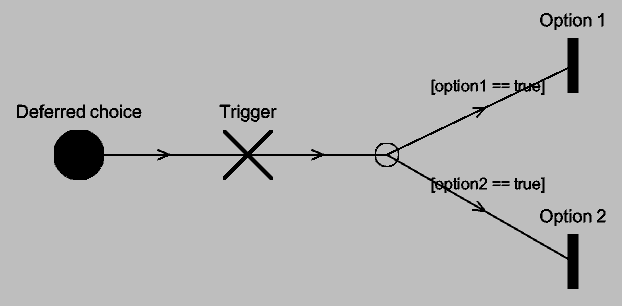
\includegraphics[scale=1.3]{fig_4_11.png}
	\caption{Deferred choice pattern}
	\label{fig:4.11}
\end{figure}

Typical implementation of deferred choice is using an AND-fork to enable all parallel branches. After one of the branches has started processing, all other branches are canceled. Since the UCM notation does not have the ability to signal for cancellation of other branches, an alternative strategy is the use of XOR-split. Figure~\ref{fig:4.11} illustrates the OR-fork implementation for the deferred choice pattern; the \emph{Trigger} is responsible for activating the proper branch, by setting $option_1$ to $true$ and $option_2$ to $false$ or vice versa. The pattern is realized as a feature in a concern and can be reused in other UCMs. One example of reuse is in the milestone pattern.

\subsection{Milestone}

The milestone pattern supports the conditional execution of a task only if a parallel process is in a given state, i.e. an activity can only be enabled if a certain milestone has been reached and has not expired yet. Different strategies exist for the implementation of the milestone pattern, and one form uses a deferred choice in the workflow. Deferred choice offers two subsequent activities and is modeled with an OR-fork within the reused Deferred Choice concern. The path to one activity is enabled only after reaching a milestone, after which the path merges prior to the deferred choice construct and the same activity can be executed repeatedly, given that the current state is still in the milestone. On the other hand, if the current state leaves the milestone, then the path to the first activity is disabled by the OR-fork, leaving only the path to the second activity.

\begin{figure}
	\centering
	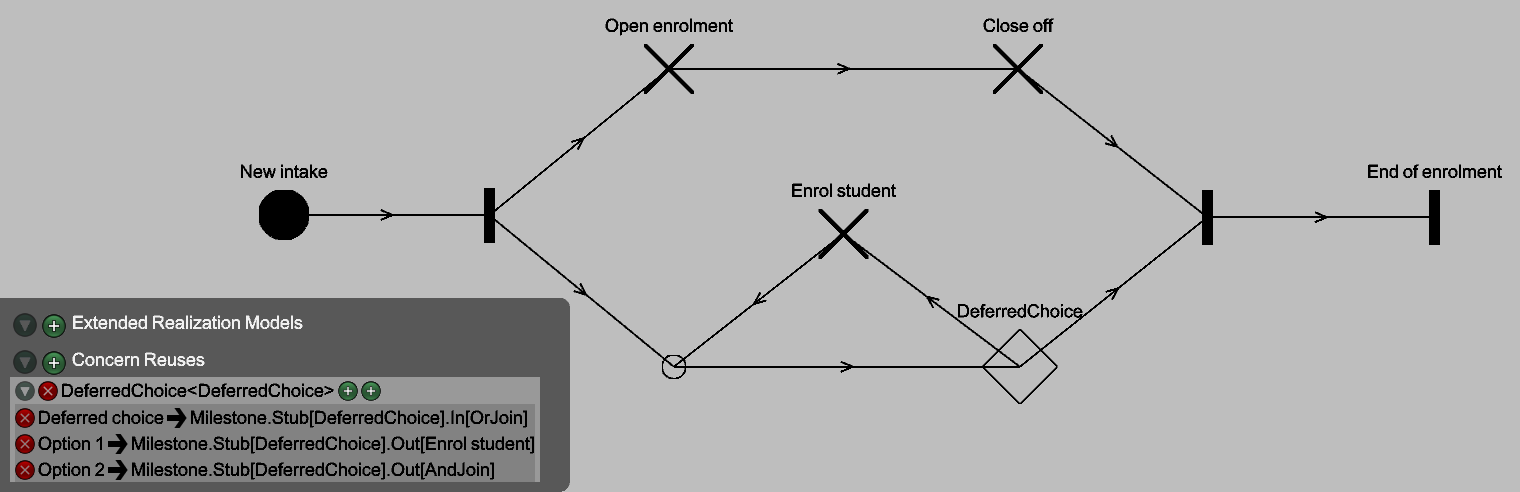
\includegraphics[scale=1.3]{fig_4_12.png}
	\caption{Milestone pattern (enrolment example)}
	\label{fig:4.12}
\end{figure}

Whereas the deferred choice pattern is modeled as a reusable concern, the milestone pattern is implemented slightly different. We took an example of student enrolment, applying the milestone pattern (deferred choice implementation), as shown in Figure~\ref{fig:4.12}. New enrolments are being accepted when the enrolment period opens (at the point of reaching a milestone) until the enrolment period closes (at the point of deadline) for a given intake. Ideally, the route to \emph{Enrol student} ($option_1$) can only be activated when the token on the other parallel path reaches \emph{Open enrolment} but before reaching \emph{Close off}. All other instances would result in inaccessible path $option_1$, leading to the only exit path available that is \emph{End of enrolment} ($option_2$).


\chapter{Conclusion} \label{ch:5}
\section{Summary}

Requirements elicitation forms a fundamental piece of software engineering and is typically performed at the initial phase of the software development process. This thesis introduces CoUCM that consolidates scenario modeling with advanced SoC, MDE, and SPL. Along with the already existing GRL support for goal modeling in CORE, the addition of UCM offers a complete URN package for requirements engineering in CORE.

The proof of concept implementation of CoUCM in TouchCORE demonstrates the project's feasibility. TouchCORE is a modeling tool that provides an intuitive interface for concern-oriented software design. Both CoUCM and RAM allow TouchCORE users to model at different level of abstractions, covering the requirements and design phases. In addition, modelers can now populate the TouchCORE library with reusable scenario models encoding essential recurring requirements concerns (e.g., functional units, workflow patterns, etc).

Limitations of the work exists, however, and serve as potential future work for improvements, which we discuss in the next section.

\section{Future Work}

The integration of UCM to CORE has not been completed yet, specifically the use of {\cls ResponsibilityRef}s to refer to a particular {\cls Responsibility} definition from multiple reference points that belong to other UCMs, as well as the use of {\cls Component}s to model the architectural structure of a system. Implementation of {\cls Component} to CoUCM poses some difficulties especially when taking model composition into account as responsibilities within a component are bound to the component. Several other model elements including waiting place, timer, failure point, and abort could be added to the CoUCM metamodel to complete the standard UCM features.

Similarly, the implementation of scenario modeling to TouchCORE is in the alpha phase. TouchCORE features such as traceability and model validation could be implemented to allow for a better scenario modeling experience. Path drawing could be improved as current implementation uses straight lines to connect path nodes; splines would work well if supported by TouchCORE GUI. One of the jUCMNav tool's features is the path traversal mechanism~\cite{kealey2007enhanced2}. If implemented in TouchCORE, this mechanism allows for UCM analysis and is particularly useful in evaluating scenario variables when traversing paths.

Supplementary work to the CORE base design is needed to allow a more seamless integration of multiple modeling languages. Since this is one of the early works (after RAM) that extends a modeling language (UCM) with concern-orientation, future addition of modeling languages to CORE can refer to this work as reference. We hope that this work would motivate future studies to further improve the CORE paradigm.


%----------------
% End Matter
%----------------
\begin{appendices}

\chapter{Complete Metamodels} \label{ch:A}
\section{CORE Metamodel}

\begin{figure}[h]
	\centering
	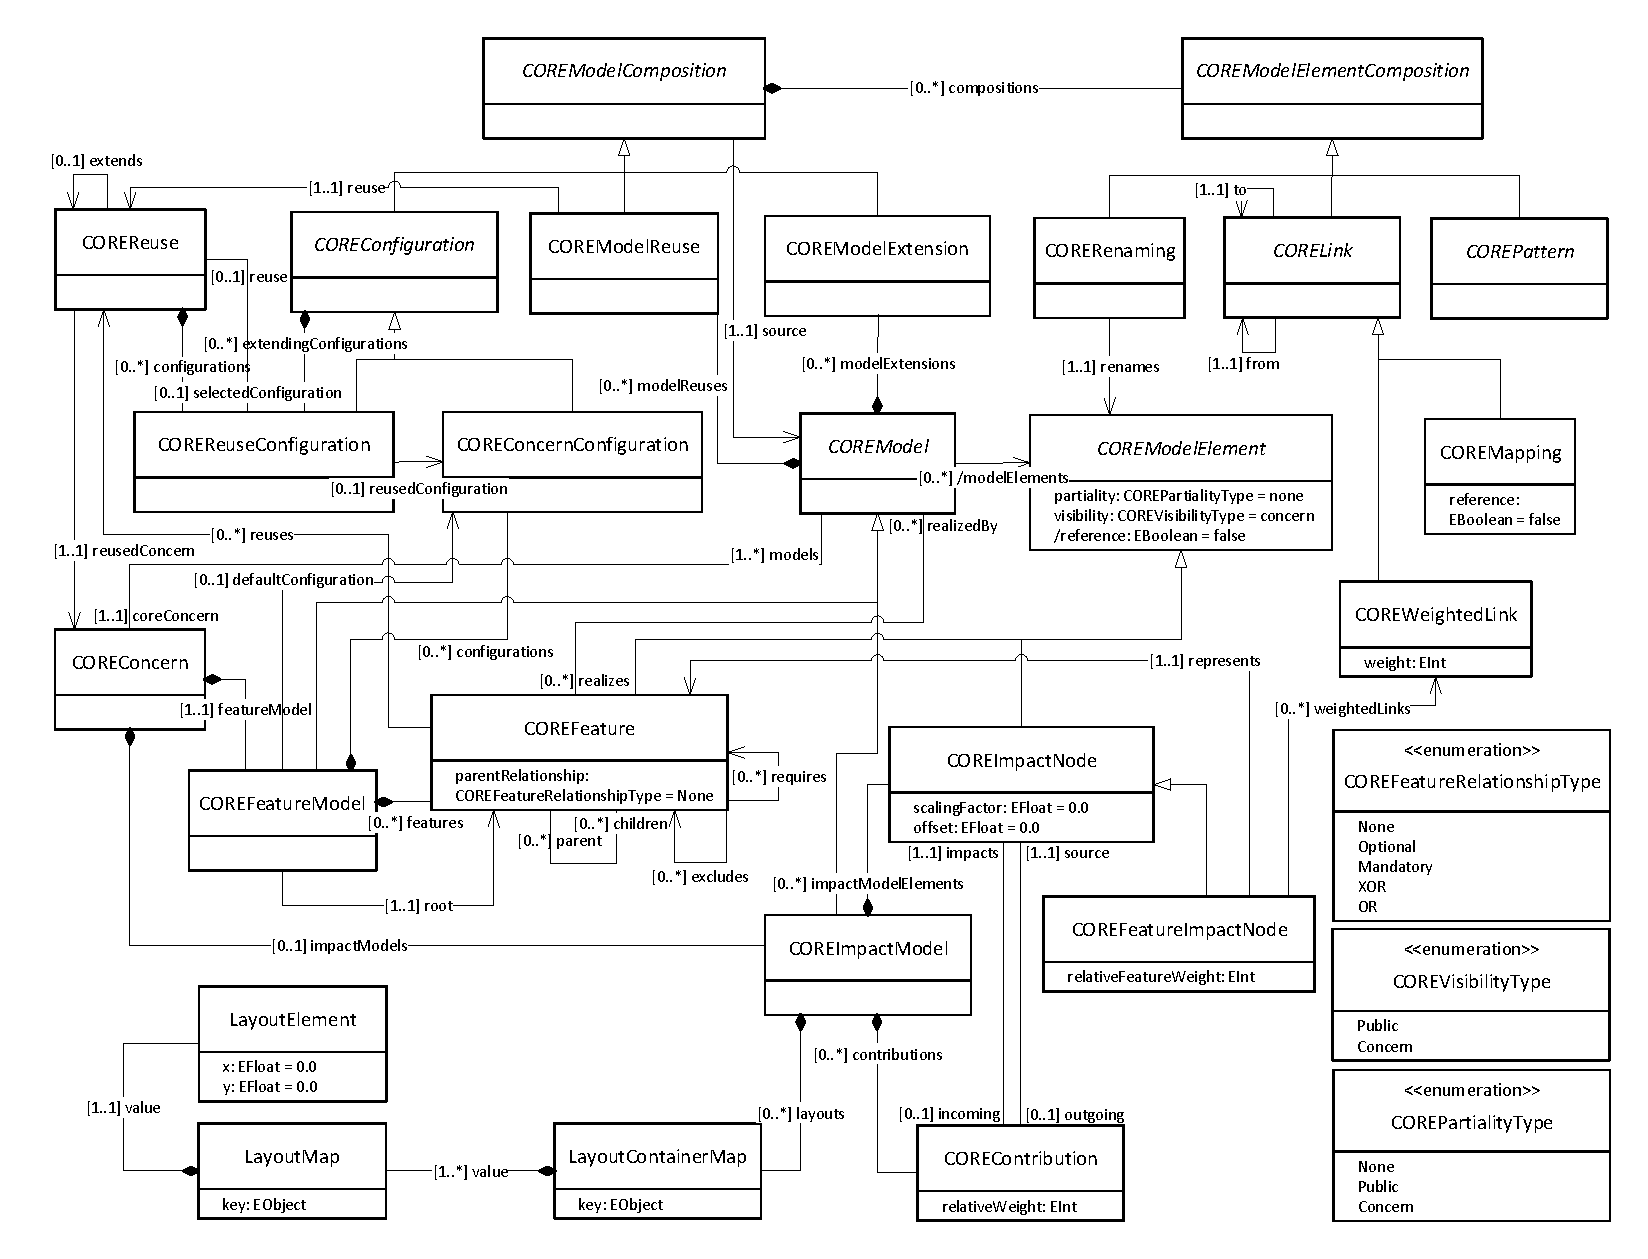
\includegraphics[scale=0.59]{fig_a_1.pdf}
	\caption{Abstract grammar: CORE metamodel overview}
	\label{fig:a.1}
\end{figure}

\section{UCM Metamodel}

\begin{figure}[h]
	\centering
	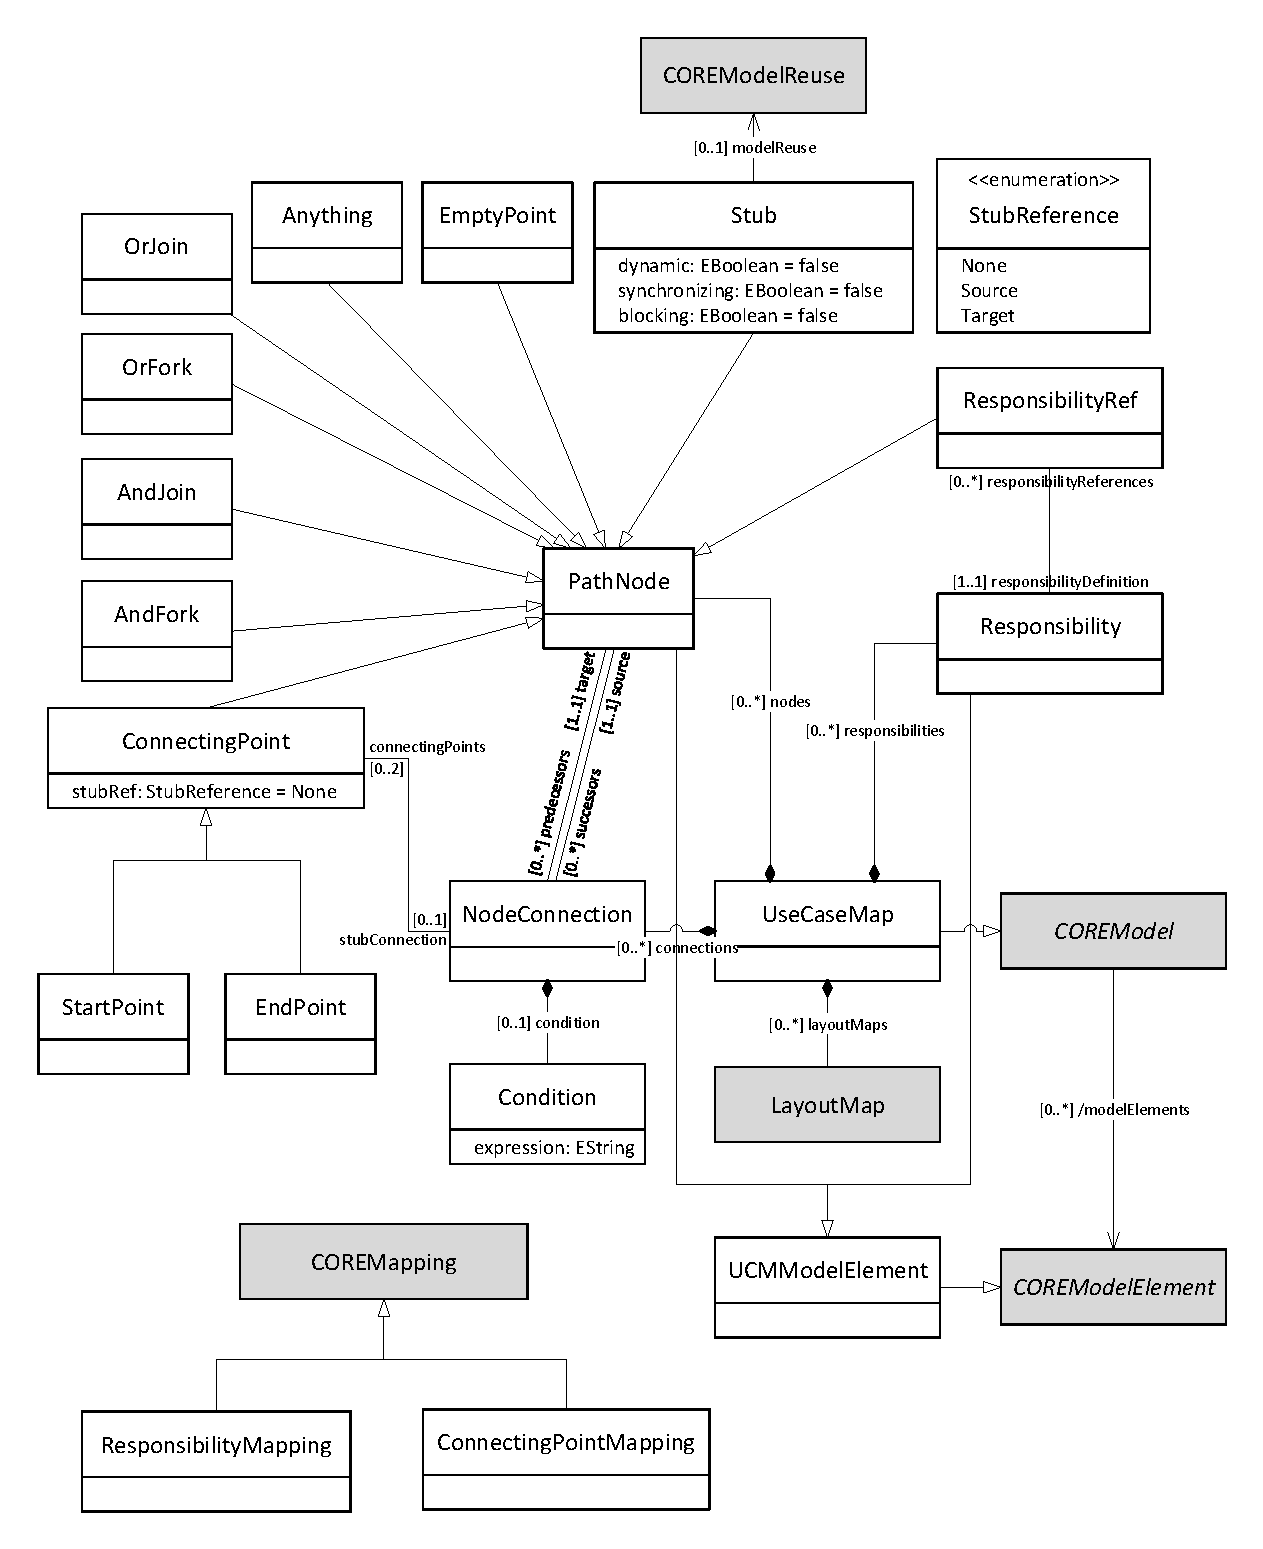
\includegraphics[scale=0.53]{fig_a_2.pdf}
	\caption{Abstract grammar: UCM metamodel overview}
	\label{fig:a.2}
\end{figure}


\end{appendices}

\renewcommand\bibname{References}
\printbibliography[heading=bibintoc]

\end{document}
